%% ----------------------------------------------------------------
%% Thesis.tex -- MAIN FILE (the one that you compile with LaTeX) MAIN REPORT
%% ---------------------------------------------------------------- 
\RequirePackage[hyphens]{url}
% Set up the document
\documentclass[a4paper, 12pt, twoside]{Thesis}  % Use the "Thesis" style, based on the ECS Thesis style by Steve Gunn
\graphicspath{Figures/}  % Location of the graphics files (set up for graphics to be in PDF format)
%\usepackage{url}
\usepackage{hyperref}
% Include any extra LaTeX packages required
\usepackage[square, numbers, comma, sort&compress]{natbib}  % Use the "Natbib" style for the references in the Bibliography\cite{Reference2}
\usepackage{verbatim}  % Needed for the "comment" environment to make LaTeX comments
\usepackage{vector}  % Allows "\bvec{}" and "\buvec{}" for "blackboard" style bold vectors in maths

\hypersetup{urlcolor=black, colorlinks=true}  % Colours hyperlinks in blue, but this can be distracting if there are many links.

\usepackage{float}
\usepackage{listings}
\usepackage{lscape}
\usepackage{multirow}
\usepackage[justification=justified,singlelinecheck=false]{caption}
\usepackage{graphicx}
%\usepackage{lineno}
%\linenumbers
%% ----------------------------------------------------------------
\begin{document}
\frontmatter      % Begin Roman style (i, ii, iii, iv...) page numbering

% Set up the Title Page
\title  {Towards Presence in Telerobotics: Real-time Image Abstraction for Virtual Reality}

\authors  {\texorpdfstring
            {Adam Melvin}
            {Author Name}
            }
\addresses  {\groupname\\\deptname\\\univname}  % Do not change this here, instead these must be set in the "Thesis.cls" file, please look through it instead
\date       {\today}
\subject    {}
\keywords   {}

\maketitle
%% ----------------------------------------------------------------

\setstretch{1.3}  % It is better to have smaller font and larger line spacing than the other way round

% Define the page headers using the FancyHdr package and set up for one-sided printing
\fancyhead{}  % Clears all page headers and footers
\rhead{\thepage}  % Sets the right side header to show the page number
\lhead{}  % Clears the left side page header

\pagestyle{fancy}  % Finally, use the "fancy" page style to implement the FancyHdr headers


%% ----------------------------------------------------------------

% The Abstract Page
%\addtotoc{Abstract}  % Add the "Abstract" page entry to the Contents
\abstract{
%\addtocontents{toc}{\vspace{1em}}  % Add a gap in the Contents, for aesthetics

The application of Virtual Reality (VR) to telerobotics is a current area of study due to a desire for the increased spacial awareness VR provides. However, attempts to implement such a system using standard teleoperation techniques result in sub-par performance and an uncomfortable experience for the user; the benefits of a VR based system are entirely eliminated. The system proposed by this project incorporates elements of data abstraction to produce abstractions of the environment. This process reduces the performance requirements of providing the user presence within the telerobot's space such that it can be achieved under reasonable budgetary constraints.

\clearpage  % Abstract ended, start a new page
%% ----------------------------------------------------------------

\pagestyle{fancy}  %The page style headers have been "empty" all this time, now use the "fancy" headers as defined before to bring them back


%% ----------------------------------------------------------------
\lhead{\emph{Contents}}  % Set the left side page header to "Contents"
\tableofcontents  % Write out the Table of Contents

%% ----------------------------------------------------------------
\lhead{\emph{List of Figures}}  % Set the left side page header to "List if Figures"
\listoffigures  % Write out the List of Figures

%% ----------------------------------------------------------------

% The Acknowledgements page, for thanking everyone
\acknowledgements{
%\addtocontents{toc}{\vspace{1em}}  % Add a gap in the Contents, for aesthetics

I would like to thank Klaus-Peter Zauner for his incredible help and support. I would also like to thank Tom Darlison and Lawrence Gray for their help and for being expert ``rubber ducks''. Finally, I would like to thank the users of the Building 16 labs for treating my rover driving around with the utmost patience.

}
\clearpage  % End of the Acknowledgements
%% ----------------------------------------------------------------

%% ----------------------------------------------------------------
\mainmatter	  % Begin normal, numeric (1,2,3...) page numbering
\pagestyle{fancy}  % Return the page headers back to the "fancy" style

% Include the chapters of the thesis, as separate files
% Just uncomment the lines as you write the chapters

\chapter{Introduction}
\lhead{\emph{Introduction}}
\label{chapter:intro}

 Whether it be within a virtual space such as in a video game or training simulation \cite{alexander2005gaming}, or within a remote real world location as in telerobotics, a feeling of presence \cite{presence} allows the user to more naturally and intuitively interact with the presented environment as if they were truly there. The desire for presence within a space that is not your own is therefore one that drives much technological innovation. In telerobotics in particular, where the aim can often be to interact with dangerous or industrial environments, intuitive control is essential to safe and effective operation.

Virtual Reality (VR) is a technology spearheaded by the video games industry for use in immersive gaming applications. Through the use of a tracked headset, giving the user the ability to freely look around a 3D space, it provide unparalleled presence within a virtual world---comparable to presence within a real, physical space \cite{loomis2016presence,McGlynn}. To be able to incorporate VR into teleoperation is therefore desirable, however, sending a video feed to the headset as if it were a normal monitor has been found to lead to motion sickness \cite{han2017design}. This is due to VR's high frame rate and low latency requirements. It's widely accepted that for a VR application to not cause motion sickness and headaches due to frame rate, it must maintain at least 90 frames per second (fps) \cite{FrameRate}; a minimum of 60 fps can also be acceptable \cite{Borg2013UsingAG}, but generally only for applications with little motion or when used by people with lower susceptibility to motion sickness. Unfortunately, to transmit 90 fps from a stereo camera rig (two images are required to perceive 3D) to the computer running the VR application has bandwidth requirements too high to be currently implementable outside the most expensive of designs.

Another consideration is the ability to look around the space independently, as this is a major factor in providing presence to the user in VR. This can be achieved by mounting the stereo camera rig on a gimbal, however to build a gimbal that is able to track the angle of the user's head accurately and with low latency is, once again, expensive and challenging \cite{DORA}; if not implemented perfectly the user would experience significant sickness and dissociation from the space.

The aim of this project is to research the use data abstraction to minimise the outlined technical issues through the design and implementation of a teleoperations sytem that incorperates it. To achieve this, the system must reduce each image down to its most essential features, reducing its size and therefore the required bandwidth significantly. Each image pair must then be transmitted to a server and combined into a single 3D model of the space that could be looked around freely through the VR headset. As the camera feed is converted to a 3D model rather than displayed directly as images, the headset could run at its maximum frame rate of 90fps even if the model is updating at a much slower rate. The use of abstractions has the capacity to allow for high presence systems, as presence in VR is not dependant on the 3D environment being an exact reproduction of the telerobot's space---only that the reproduction is consistent and comfortable to view. 

\begin{figure}[H]
    \begin{center}
      \includegraphics[width=0.7\textwidth]{Figures/Outline.jpg}
      \caption[System Outline]{System Outline. It can be seen that the scene the rover's cameras are observing (top left) is within the VR environment (top right) as a simple abstracted 3D representation.}
      \label{fig:outline}
    \end{center}
\end{figure}

The system (cf. Figure \ref{fig:outline}) consists of two platforms: a server (Chapter \ref{chapter:server}) that runs a VR environment and reads user input from an Xbox 360 controller, and a rover platform (Chapter \ref{chapter:rover}) that is controlled from said environment and supplies the abstracted images that the 3D model in the environment is built from. The rover (Figure \ref{fig:marvin}) is a simple drivable platform with a stereo camera gimbal mounted on it (adapted from one produced by previous students \cite{gimble}). The server is a powerful PC running Windows 10 \cite{windows} and a HTC Vive \cite{Vive}. The data abstraction algorithm the system uses is novel, so its design and development is initially discussed in isolation (Chapter \ref{chapter:abstract}), and then its implementation within the system explained as part of the rover implementation (Chapter \ref{chapter:rover}).

\begin{figure}[H]
    \begin{center}
      \begin{tabular}{ c }
        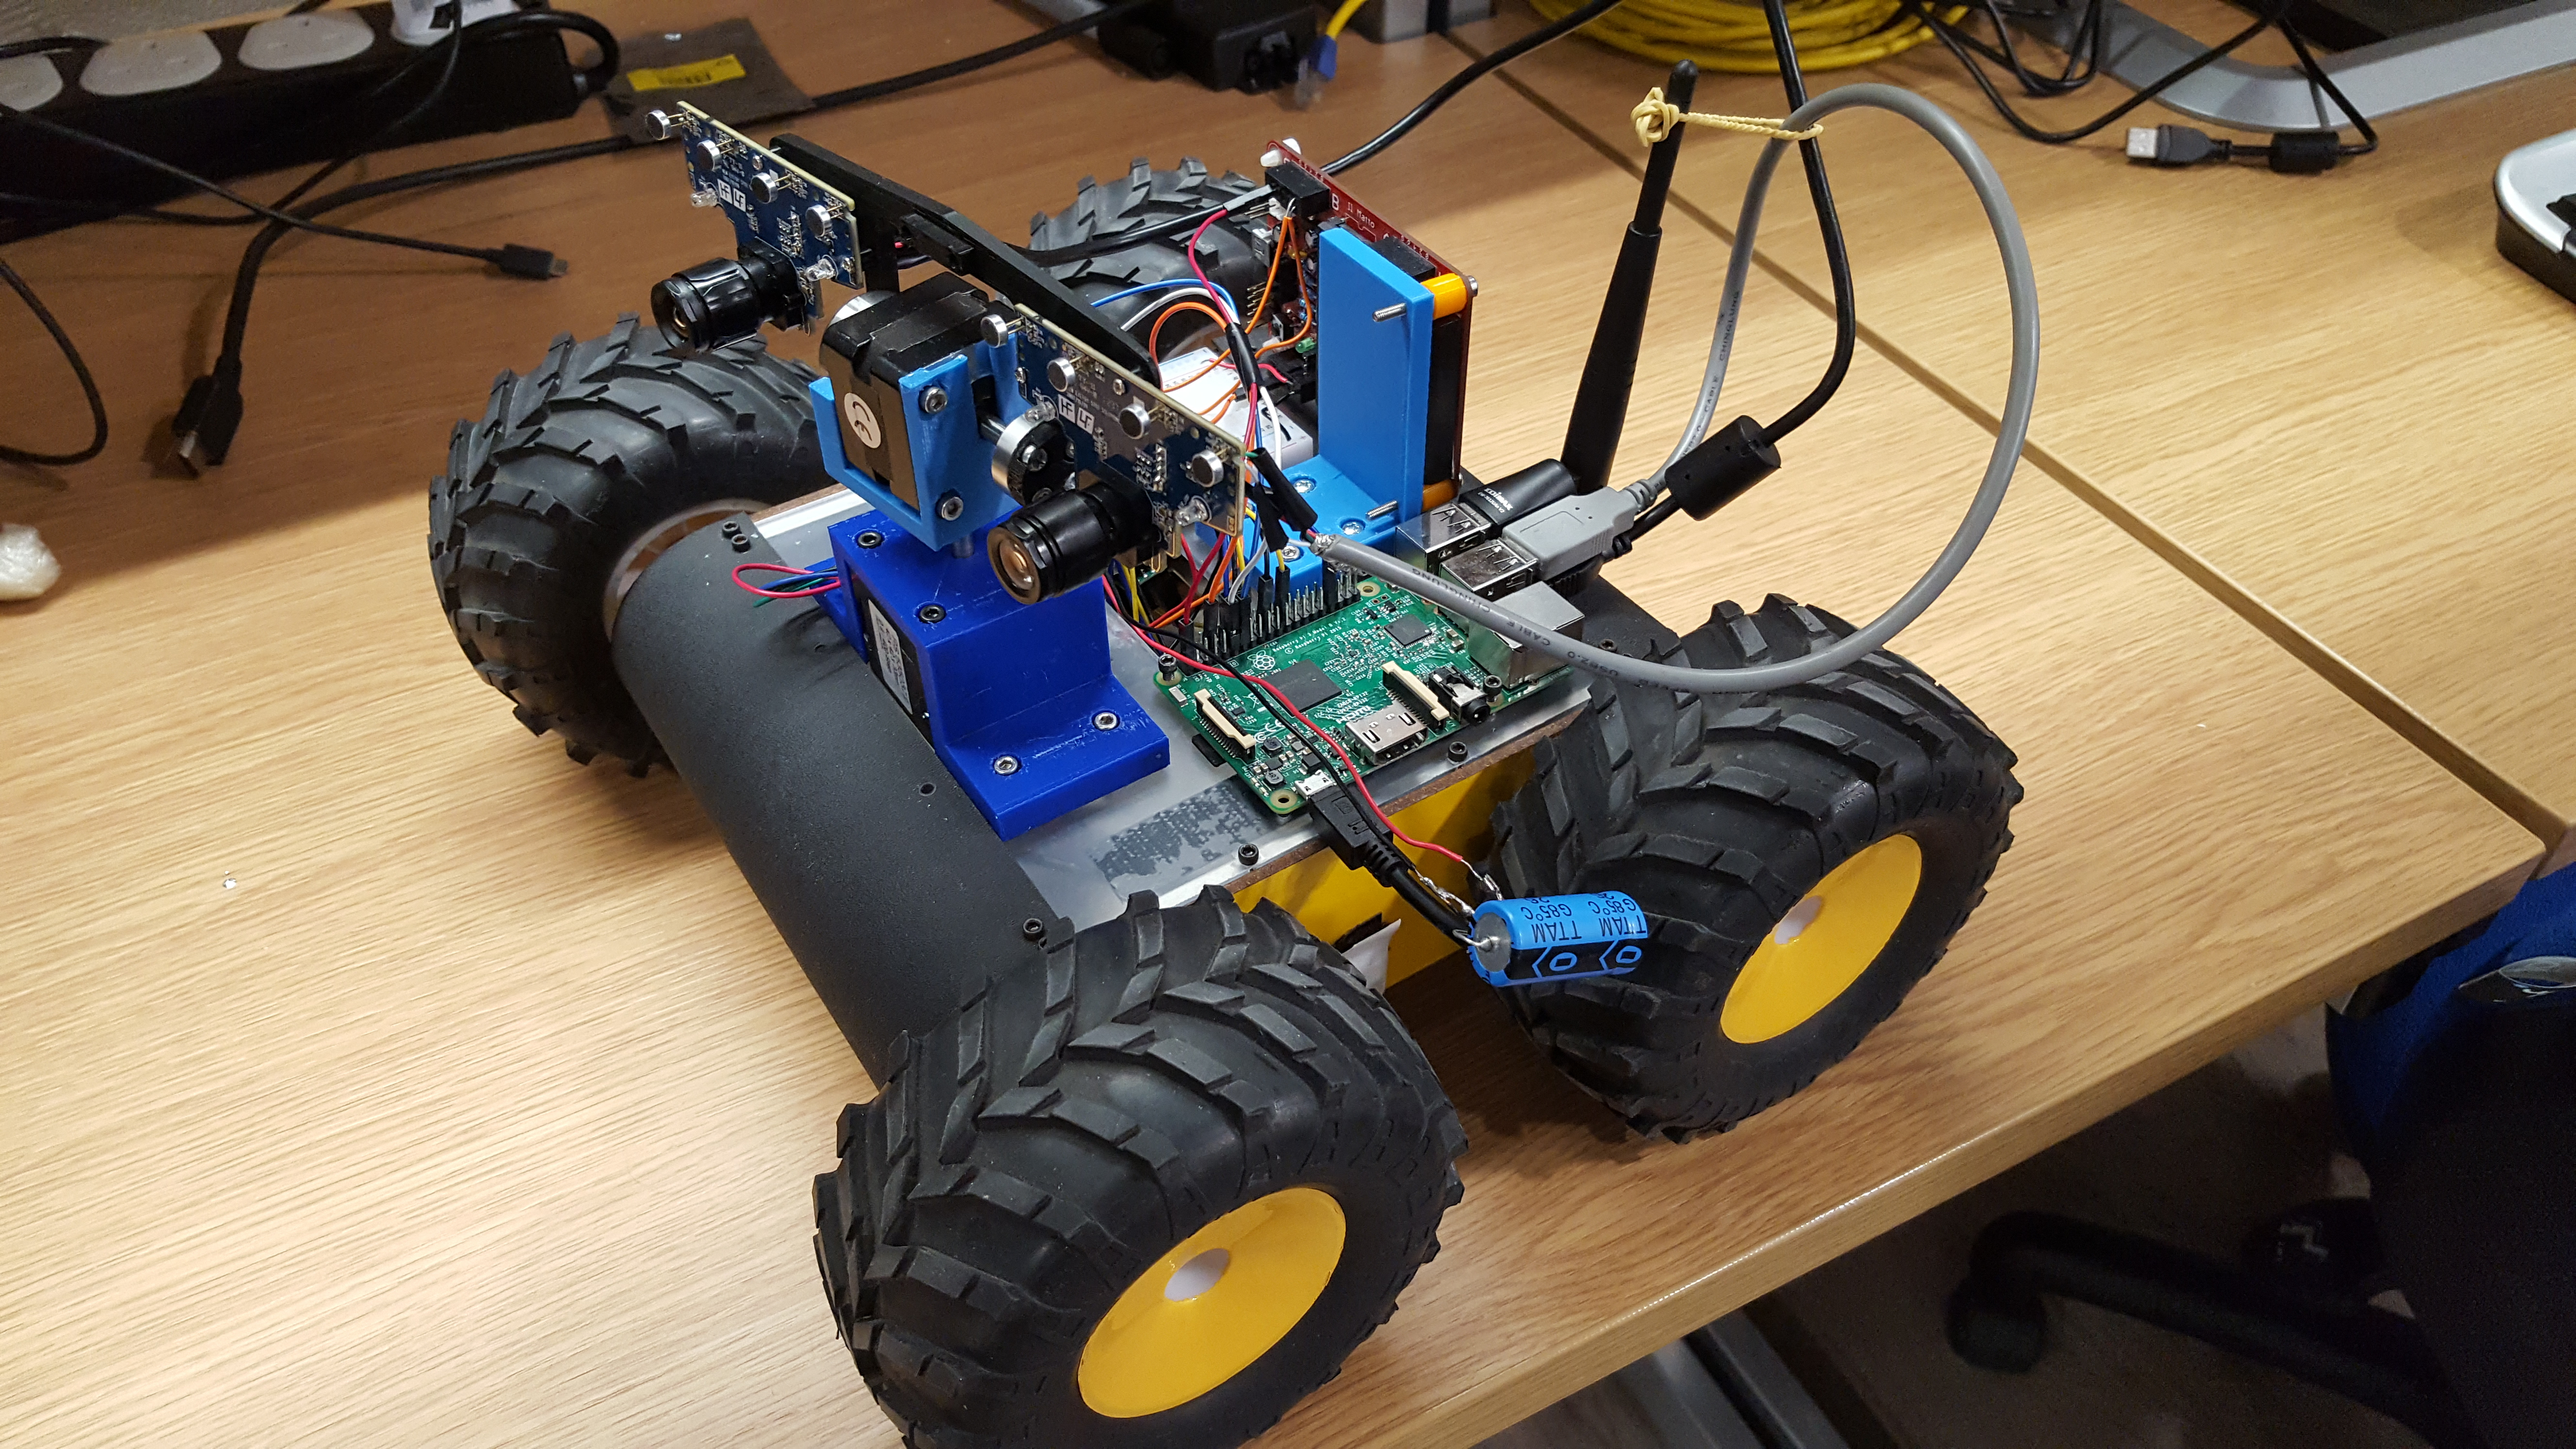
\includegraphics[width=0.65\textwidth]{Figures/marvin.jpg} \\
        \includegraphics[width=0.65\textwidth]{Figures/marvinF.jpg} \\
        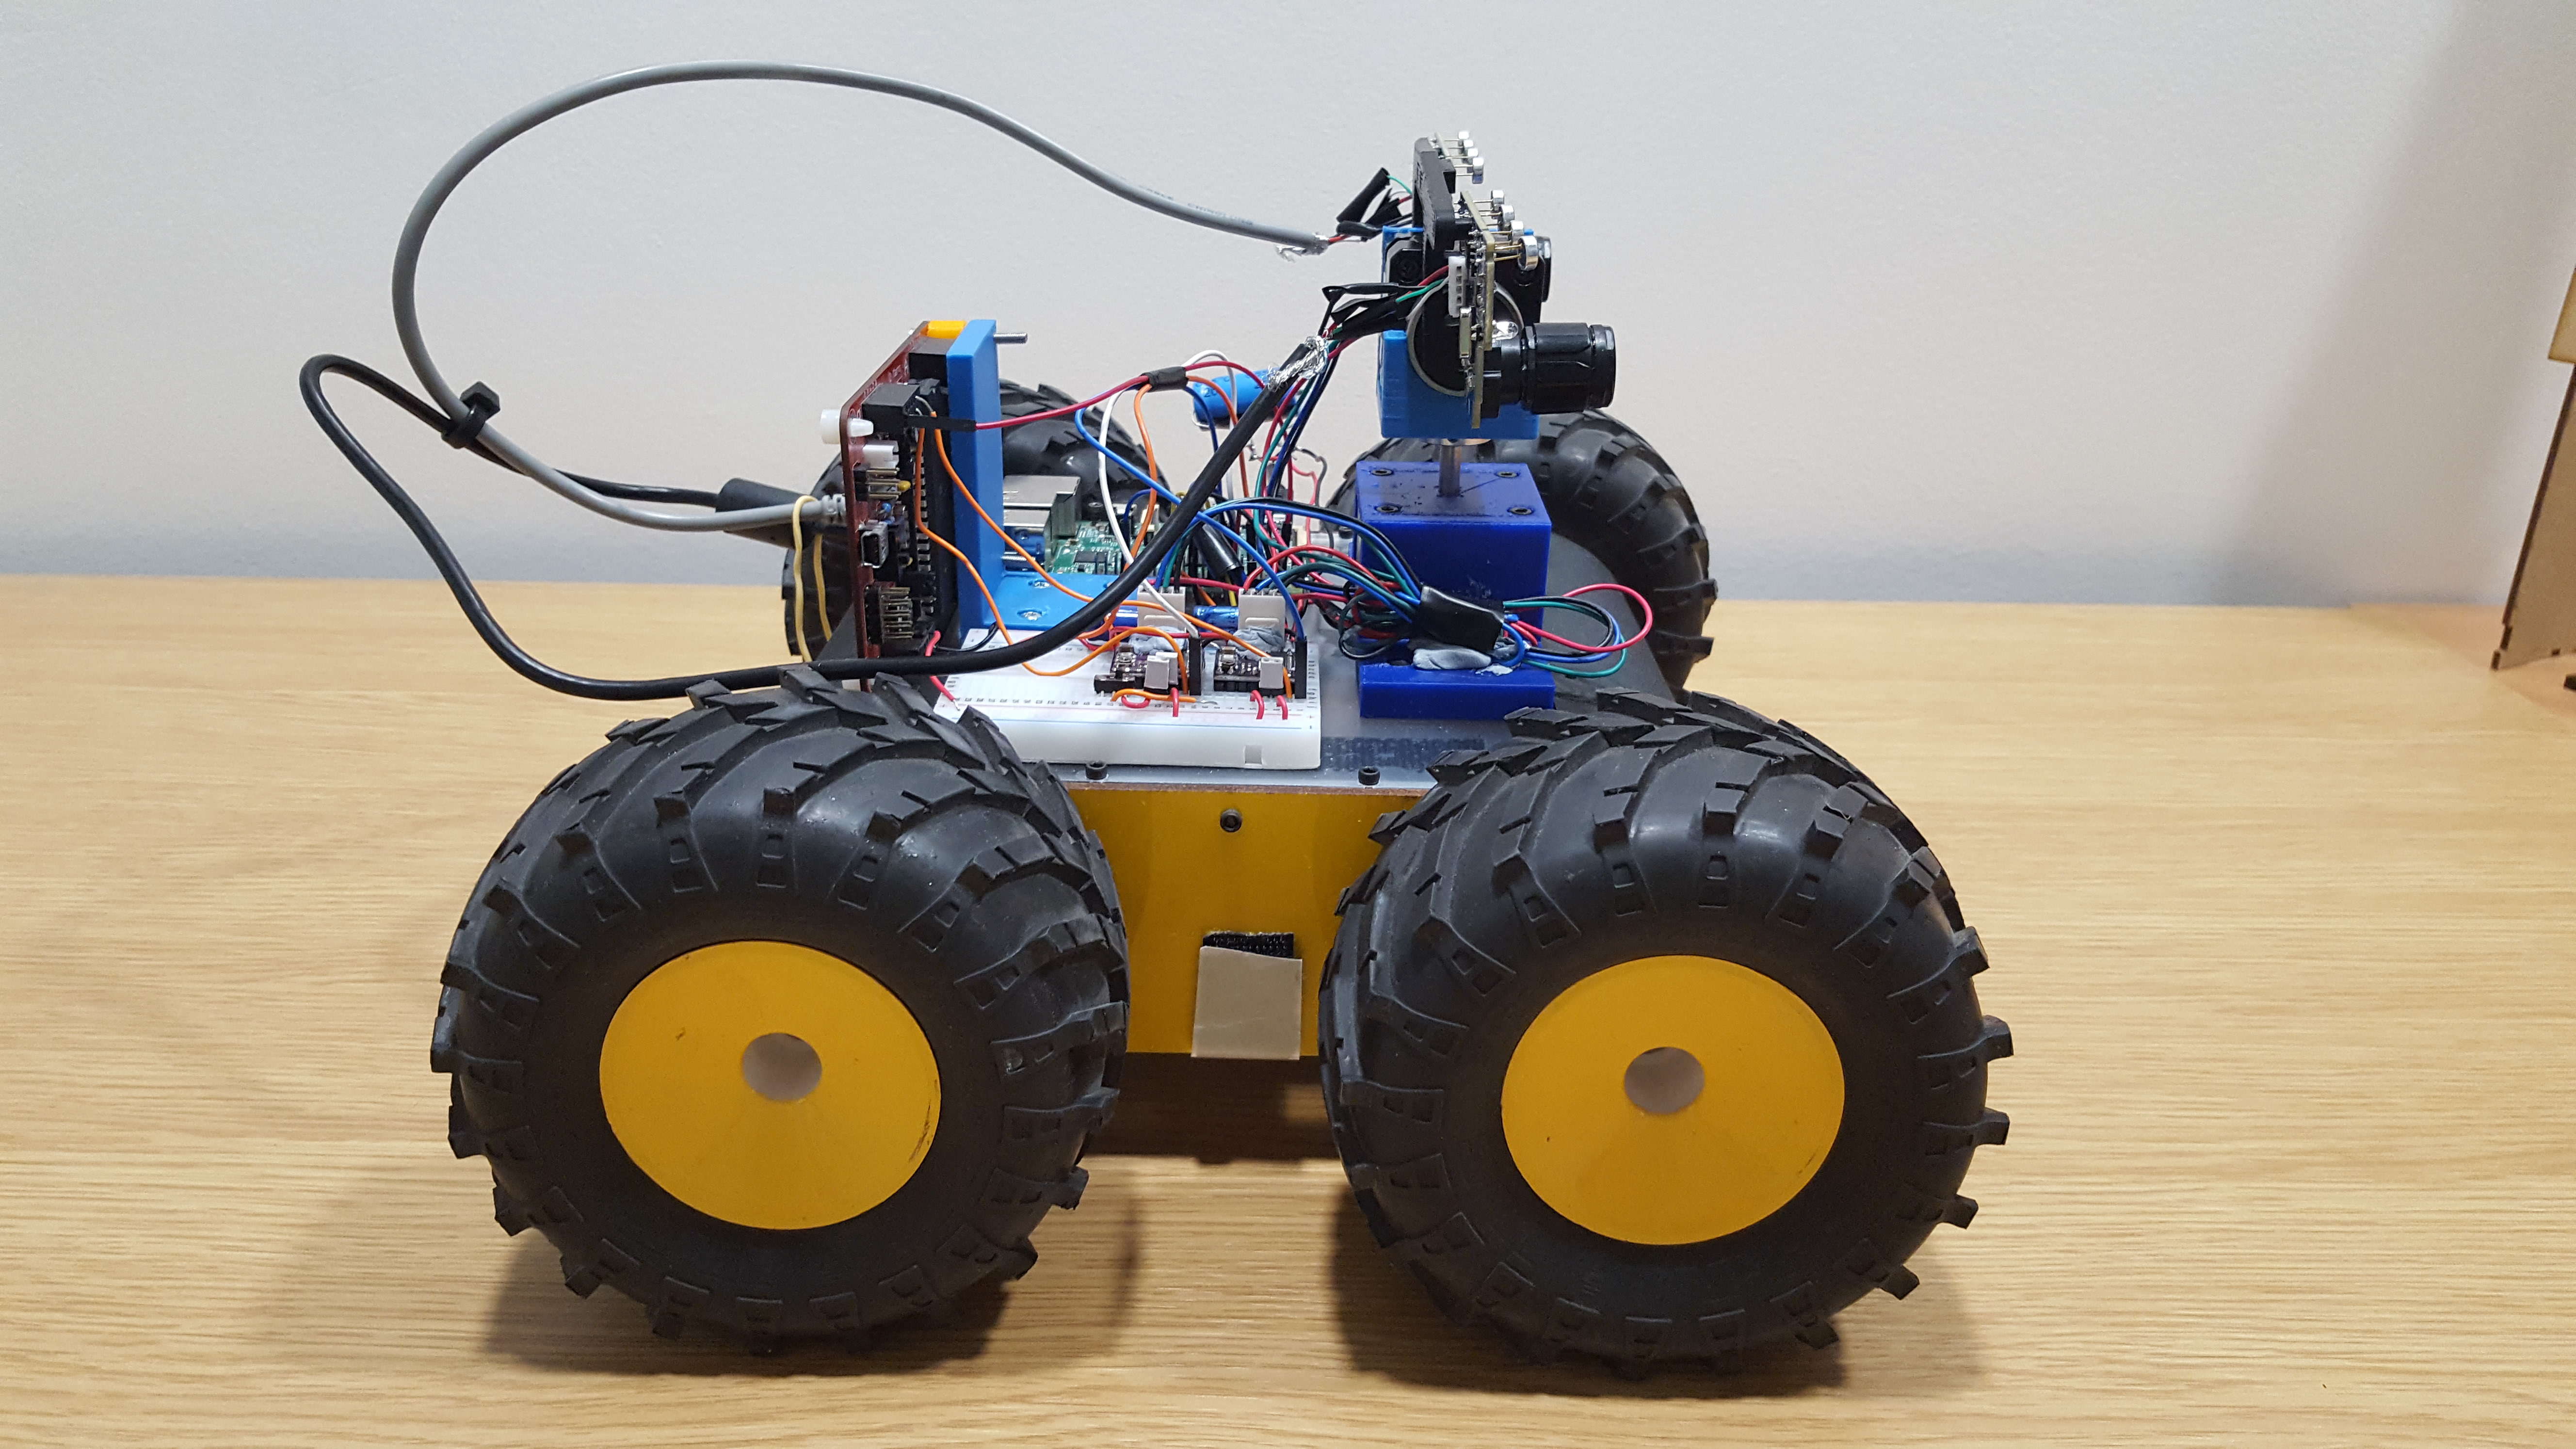
\includegraphics[width=0.65\textwidth]{Figures/marvinS.jpg} \\
        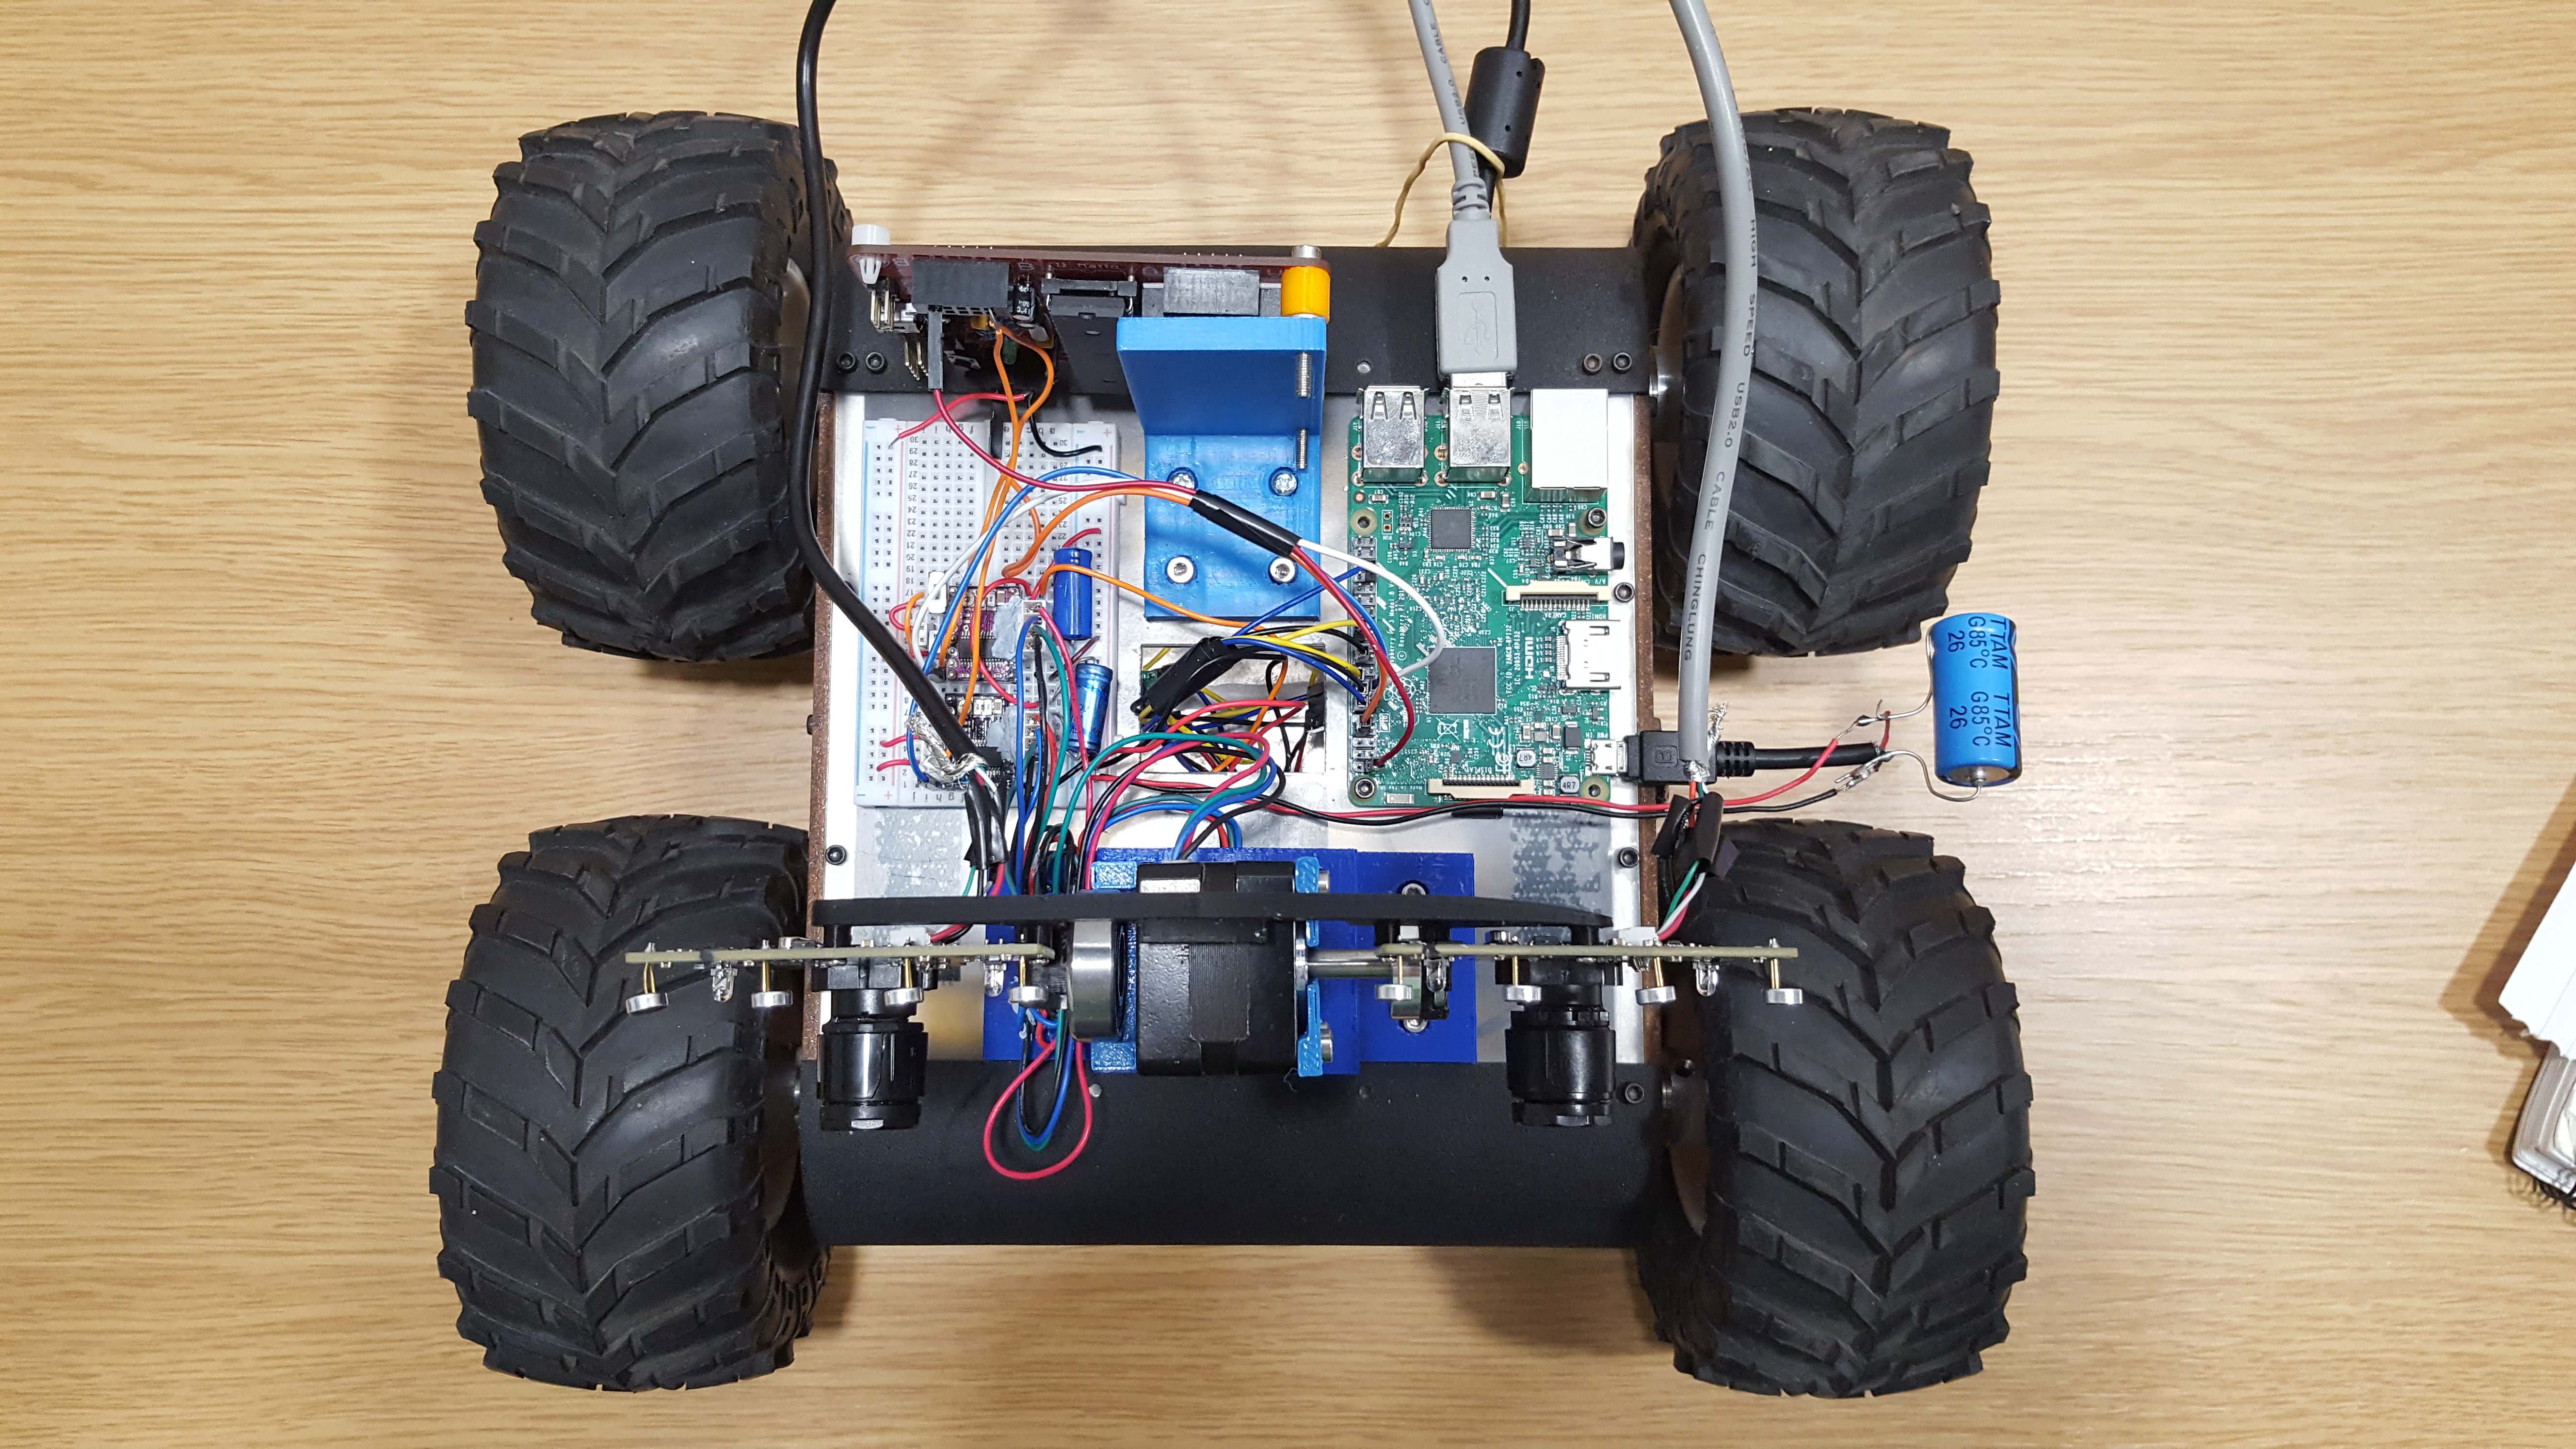
\includegraphics[width=0.65\textwidth]{Figures/marvinT.jpg}
      \end{tabular}
      \caption[Rover Pictures]{Rover Pictures.}
      \label{fig:marvin}
    \end{center}
\end{figure} % Introduction

\chapter{Background}
\lhead{\emph{Background}}

\section{Virtual Reality}

The term Virtual Reality (VR) refers to the generation of a 3D environment that can be interacted with by a user in a realistic fashion, with the aim of immersing the user in the environment as if it were the real world \cite{WhatVR}. While there are a large array of systems that can be considered VR, whenever the term is used in this report it is only referring to the head-mounted display (HMD) systems that have become popular in recent years with the release of the Oculus Rift \cite{Oculus} and the HTC Vive \cite{Vive} (Figure \ref{fig:Vive}); these are both consumer grade systems that are aimed at the immersive gaming market.

\begin{figure}[H]
    \begin{center}
    \begin{tabular}{ c c }
        \includegraphics[width=0.4\textwidth]{Figures/vive.png} &
        \includegraphics[width=0.4\textwidth]{Figures/vive2.png}
    \end{tabular}
    \caption[HTC Vive]{HTC Vive. Pictures of the Vive headset, reproduced from \cite{Vive}.}
    \label{fig:Vive}
    \end{center}
\end{figure}

HMD based systems display different images for each eye to provide the user with a sense of depth within the 3D environment, making the headset effectively operate like a pair of binoculars into the virtual world. The headset is also tracked in 3D space, and this movement translated into the 3D environment with very low latency. These features, among others, are all implemented with the aim of providing the user with presence within the virtual space that is comparable to observing the real world.

Due to its availability at the University of Southampton and in my own home, the HTC Vive was used as the VR device in the development and implementation of the teleoperations system discussed in this report. 

\section{Telerobotics}

A telerobot is a robot controlled from a distance by a human operator \cite{NAP4761}. Telerobots are typically developed to undertake activities within environments that are too dangerous or costly for humans to work in, examples being the extensive telerobotics research for tasks such as deep-space exploration \cite{fong2017interactive}, deep-sea exploration \cite{huvenne2018rovs}, and handling radioactive materials \cite{smith2017radiation}.

\subsection{VR in Telerobotics}
\label{subsection:VRTele}

The use of HMDs in teleoperations is not a new concept; NASA's Robonaut 2 was sent to the International Space Station in 2011 and can be controlled through a headset that displays the output of the robot's head cameras \cite{Robonaut}, and flying drones by First Person View (FPV), an analogue video feed transmitted over radio to a HMD, is very popular \cite{FPV}. However, these systems are either incredibly expensive (Robonaut 2 is worth millions of dollars) or very limited (FPV systems send one, low quality, video stream over a short distance), and all have the motion sickness issues discussed in the introduction. While stereo camera FPV systems have been developed, so the user has depth perception and better presence in the drone's view, the motion sickness problem remains the major drawback of HMD based teleoperations systems \cite{2FPV}.

As previously established, motion sickness in VR is mitigated through high frame rates and low latency. However, typically VR based teleoperations systems are direct VR systems, so they display the video feeds produced from the device's cameras directly in the headset. This entirely ties the frame rate and latency of the headset to the capabilities of the video transmission system, and only the most expensive and complicated systems will meet the strict requirements for comfortable VR and the spacial presence desired.

An alternate option to a direct system is an indirect system. This is one in which the video feed is abstracted from the headset in some way in the hope of providing improved comfort and awareness. Indirect systems can come in a variety of forms, such as placing the video feed on a virtual screen in the VR environment and controlling the robot using virtual controls laid out infront of the screen \cite{lipton2018baxter}, or a 3D map generated from a multi-line LiDAR and IMU \cite{wang2017novel} (Figure \ref{fig:VRTele}). These examples show the potential of indirect systems as a solution to VR based teleoperations, however neither of them provide true presence within their respective robots' spaces. The research into indirect systems is currently minimal; this project aims to expand on this research with the development of its novel system.

\begin{figure}[H]
    \begin{center}
    \begin{tabular}{ c c }
        \includegraphics[width=0.45\textwidth]{Figures/homun.png} &
        \includegraphics[width=0.5\textwidth]{Figures/lidar.png}
    \end{tabular}
    \caption[Indirect VR teleoperations examples]{Indirect VR teleoperations examples. A virtual control room based system (left) and a LiDAR 3D map based system (right), reproduced from \cite{lipton2018baxter} and \cite{wang2017novel}.}
    \label{fig:VRTele}
    \end{center}
\end{figure}

\section{Data Abstraction}
\label{Subsection:abstract}

\textit{Data abstraction} is the phrase that will be used in this report to describe the act of reducing an image down to only its most essential elements. It is similar in concept to an artist sketching a scene instead of attempting a full drawing. Comparing the concept to data compression is apt, as both aim to reduce the file size of the image, however data abstraction takes a very different approach to solving the problem than standard compression algorithms.

Data compression is the storing of information using a more space efficient encoding \cite{compression}. While some information is lost during lossy compression, the aim regardless of the algorithm used is to retain as much of the original information as possible. In contrast, the aim when utilising data abstraction is to discard all the information that is unnecessary to fulfilling the image's purpose. For example, if all that is required of an image is that basic shapes can be identified, then only the information on the boundaries of the shapes is necessary; the rest of the image can be discarded. An implementation of data abstraction can be seen in Figure \ref{fig:abstraction3rdyear}.

%\caption[My figure Title.]{My figure Title. Details how it was made. What is the point? Reproduced from}

\begin{figure}[H]
    \begin{center}
      \includegraphics[width=0.6\textwidth]{Figures/abstraction3rdyear.png}
      \caption[Data Abstraction Example]{Data Abstraction Example. This is the abstraction of an aerial photograph of London, reproduced from \cite{abstraction3rdyear}}
      \label{fig:abstraction3rdyear}
    \end{center}
\end{figure}

\section{Sobol Sequences}
\label{Subsection:sobol}

Sobol sequences are quasi-random sequences that were introduced to aid in approximating integrals. The aim is to form a sequence of points that are evenly spread across an S-dimensional unit cube \cite{joe2008constructing}. This provides a much more even spread of points across the chosen space than can be produced from a pseudo-random number source (Figure \ref{fig:Sobol}). The code used in this project to produce these sequences was created by Leonhard Gr\"unschlo\ss\space \cite{CodeSource}.

\begin{figure}[H]
    \begin{center}
    \begin{tabular}{ c c }
        \includegraphics[width=0.33\textwidth]{Figures/Pseudorandom_sequence_2D.png} &
        \includegraphics[width=0.33\textwidth]{Figures/Sobol_sequence_2D.png}
    \end{tabular}
    \caption[Comparison of pseudo-random and quasi-random sequences]{Comparison of pseudo-random and quasi-random sequences. 256 points from a pseudo-random generator (left) and 256 points from a Sobol sequence (right), reproduced from \cite{SobolWiki}.}
    \label{fig:Sobol}
    \end{center}
\end{figure}

\section{Computer Vision}

Computer vision is the automatic analysis of images and extraction of the useful information they contain \cite{CVDef}. A raw image is simply a large matrix of colour values, so for a computer to take action based on the contents of an image it must be able to recognise features using analysis of this data. Doing so involves many different techniques such as statistical pattern classification and geometric modelling \cite{ballard1982computer}. All computer vision methods in this project are implemented using the OpenCV libraries, and the example programs provided with them used as starting points for development \cite{OpenCV}.

\subsection{Edge Detection}
When attempting to recognise the features of an image, knowing the locations of the edges of objects within the scene is often very useful. An edge is defined as a significant local change in intensity, usually due to a discontinuity in either the intensity or its first derivative \cite{jain1995machine}. There are many algorithms available that will detect the edges of an image from the locations of these discontinuities. When the most popular algorithms (Laplacian of Gaussian, Robert, Prewitt, Sobel, and Canny) are compared \cite{maini2009study}, the most effective in almost all scenarios is Canny edge detection \cite{canny1986computational}, therefore this is the algorithm utilised in this project. Canny edge detection is demonstrated in Figure \ref{fig:canny1}.

\begin{figure}[H]
    \begin{center}
      \includegraphics[width=0.9\textwidth]{Figures/canny2.png}
      \caption[Canny Edge Detection Example]{Canny Edge Detection Example. Simple edge detection program applied to a fairly detailed photo of Messi, to demonstrate its effectiveness even with more complex images. Figure taken from an OpenCV Canny tutorial \cite{Canny1Source}.}
      \label{fig:canny1}
    \end{center}
\end{figure}

\subsection{Flood Fill}

Flood fill algorithms determine the area connected to a given cell (the seed point) in a multi-dimensional array that have similar intensity values for the purpose of filling them with a chosen colour \cite{FloodFill}. This is a technique that is not only useful in image processing, but also for many other fields such as in passive acoustic monitoring where finding the area connected to a given node can be useful as part of tracking in 4D space (x,y,z,time) \cite{nosal2008flood}. A demonstration of flood fill has been presented in Figure \ref{fig:EgFloodFill}.

\begin{figure}[H]
    \begin{center}
    \begin{tabular}{ c c }
        
\includegraphics[width=0.35\textwidth]{Figures/blox.jpg} &
        \includegraphics[width=0.35\textwidth]{Figures/bloxFilled.jpg}
    \end{tabular}
    \caption[Example of Flood Fill]{Example of Flood Fill. The original image (left) was provided by OpenCV \cite{OpenCV}. The right image is the result of flood filling from the top left corner.}
    \label{fig:EgFloodFill}
    \end{center}
\end{figure}

\subsection{Depth Mapping}
\label{subsection:depth}

The main component in the human brain's perception of 3D is the identification of disparity between the locations of objects in the 2D images being produced by our eyes \cite{qian1997binocular}. The greater the difference in the horizontal placement of an object between the images, the closer the object to the observer. This technique can be used in computer vision to produce depth/disparity maps. Depth maps display differences in depth as a gradient from white to black (Figure \ref{fig:depthmap}), and can be produced using a variety of difference algorithms. The most common are block matching algorithms, which use simple geometry and the matching of blocks of pixels horizontally in the 2 images to calculate depth \cite{linda2001stockman}. For these algorithms to locate the same object in different places in the 2 images, the cameras taking them must be calibrated to rectify any distortion due to the lenses \cite{distort} or discrepancies in the mounting that would cause them to be out of line \cite{stereocal}.

\begin{figure}[H]
    \begin{center}
      \includegraphics[width=0.8\textwidth]{Figures/depthmap.png}
      \caption[Depth Mapping Example]{Depth Mapping Example. A stereo pair of images, with their exact disparity map bottom left and a disparity map produced by a dense disparity map estimation algorithm bottom right- reproduced from \cite{deptheg}.}
      \label{fig:depthmap}
    \end{center}
\end{figure}

\section{Wireless Communication}

The different methods of wireless communication available for a telerobotics system have varying requirements and benefits. For instance, the analogue video transmission found in FPV drone flying (as mentioned in Section \ref{subsection:VRTele}) is low latency at the expensive of video quality, range, and communication outside of line of sight. This is fine for flying a drone from the ground just below it, but would not be adequate for controlling a telerobot from a VR headset in a completely different room as is the aim of this project. A better choice of communication method would be over Wi-Fi, as a Wi-Fi router can easily allow communication across a whole building (or in the case of university Wi-Fi - a whole campus). The trade off is an acceptable increase in latency.

The two main protocols available for Wi-Fi communication are TCP (Transmission Control Protocol) and UDP (User Datagram Protocol). TCP is a connection-oriented protocol, so uses handshaking to guarantee reliable and ordered transfer of data \cite{fall2011tcp}. The trade off to this is that the handshaking slows down the process of communication. If the priority of a system is speed over packet reliability and ordering, UDP may be a better choice. There is no checking in UDP, so there is no guarantee that the packets will arrive but they can be sent with minimal overheads \cite{postel1980user}. The chosen protocol for this system is UDP, as images not arriving in the correct order and the ocassional loss of packets would not have a significant effect on the functionality of the system in comparison to the usability improvement a reduction in latency provides. % Background 

\chapter{System Overview}
\lhead{\emph{System Overview}}
\label{chapter:system}

The telerobotics system presented (Figure \ref{fig:system}) consists of a fairly complex image processing pipeline running alongside a simple control system, with very little interaction between the two. The pipeline starts with the 2 cameras on the rover taking a picture each as close to simultaneously as possible. These images then get abstracted down to edge detected sets of lines, with a set of colours also generated from "Image 1" to combine with its edge detected version later on. These 3 pieces of data are then compressed into a single packet and transmitted via UDP to the server. The server splits them up again and produces a depth map from the 2 edge detected images. This depth map is passed to the 3D Environment to be used to produce a 3D model of the space the cameras were looking at. The server also combines the "Colour Data" and "Edge Detected Image 1" into a full coloured abstraction, which is overlaid onto the 3D model in the 3D environment. This environment is finally observed in the VR Headset.

The rover is controlled from an Xbox 360 controller that is connected to the server. Control inputs for driving the rover, gimble orientation, and parameters for the data abstraction (the only crossover between the control and image processing components) are transmitted to the rover at a fixed rate over UDP. It should be noted that in this system there is no connection between the orientation of the headset and gimble. The focus of this project was on providing the image processing foundations for future high presence systems, therefore the control system is the minimum required to explore the effectiveness of the chosen approach.

\begin{figure}[H]
    \begin{center}
      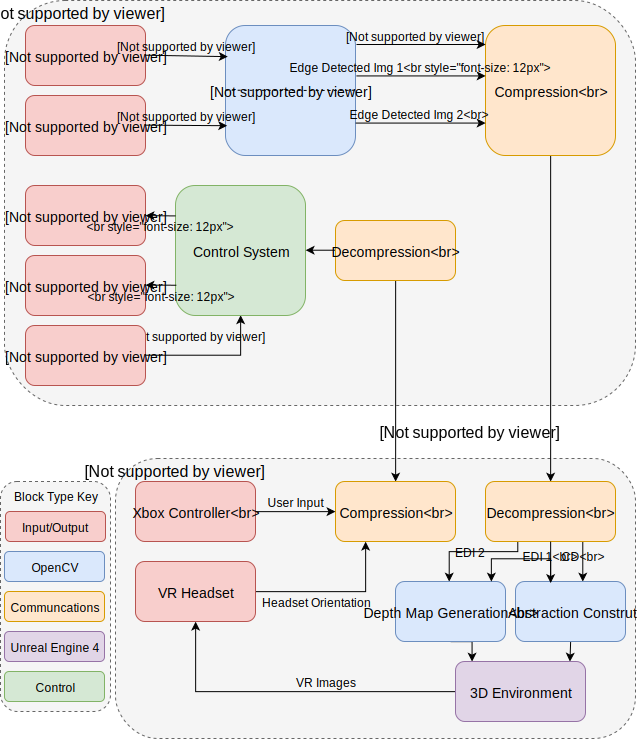
\includegraphics[width=0.8\textwidth]{Figures/System.jpg}
      \caption[System Overview Block Diagram]{System Overview Block Diagram. The red blocks represent input/output, the blue blocks represent image processing steps, the yellow blocks represent communications, and the purple block represents the 3D environment.}
      \label{fig:system}
    \end{center}
\end{figure} % System Overview

\chapter{Abstraction Algorithm Development}
\lhead{\emph{Abstraction Algorithm Development}}
\label{chapter:abstract}

In Section \ref{Subsection:abstract} we defined data abstraction as the reduction of an image down to only its most essential elements. What these essential elements are depends on the application, leading to a large range of possible methods and results. In this implementation of data abstraction, the aim is to be able to navigate a rover from the images, therefore the most important elements of each image are the size and shape of the objects in it. It is possible to convey the rough shape of an object by presenting its outline, therefore leading to edge detection being chosen as the first step of the algorithm. Identification of objects, while possible using edges alone, is significantly easier when colour is provided. However, most of the colours in an image do not aid in object identification; one colour (preferably the average colour) for each object in the scene is sufficient. This leads to the algorithm presented in Figure \ref{fig:process} and examples of the abstractions it produces can be seen in Appendix \ref{Appendix:demo}.

\begin{figure}[H]
    \begin{center}
      \includegraphics[width=0.75\textwidth]{Figures/Abstraction.jpg}
      \caption[Data Abstraction Algorithm Process]{Data Abstraction Algorithm Process. The left half is explained in the "Edge Detection Process" section, and the right half in the "Colour Averaging" section, both located below.}
      \label{fig:process}
    \end{center}
\end{figure}

This section is presented in the context of the entire process occurring on a single computer; when incorporated into the final system, the whole process is undertaken on the rover apart from the "Fill dilated image with average colour" block, which is implemented on the server in its own loop through every sobol point ("Coloured Abstraction Construction" on Figure \ref{fig:system}). It is also worth noting that this chapter is concerned with the algorithm's ability to produce recognisable abstractions under reasonable resource constraints, and not the file sizes of said abstractions. The file sizes it is capable of producing will be covered as part of the discussion of the full system's communications protocol later on in Section \ref{Subsection:comms}.

\section{Edge Detection Process}

Canny edge detection was implemented using the Canny function provided by OpenCV \cite{OpenCV}. The image is first converted into a grayscale format, as the edge detector detects large changes in intensity and not colour. The image is then blurred to remove any unnecessary edges and noise that may be picked up. The edge detection is applied, producing white lines representing the edges on a black background. The output of the edge detection is finally dilated to make the lines thicker and bridge the gaps between the lines that are very close together. This is done to reduce the number of lines produced by areas that are dense with detail such as hair and foliage and to bridge the gaps between lines that are close together, increasing the likelihood of defined shapes being created that can be easily flood filled later.

\section{Colour Averaging}

Flood filling was chosen as the method for applying colour to the edge detected image, as it is an effective method for filling spaces of unknown size and shape that are defined by high contrast boundaries. The OpenCV flood fill function requires a seed point to start flooding from, a colour to fill with, and parameters for the filling itself (unchanged from the defaults provided by the OpenCV documentation \cite{opencvffilldemo}).

\subsection{Seed Point}

Finding the points to flood fill from is a challenge, as each image will have a different number of spaces to be filled and the spaces can be anywhere. Three different methods were attempted to solve the problem. The first was an attempt to use OpenCV's contour functionality to turn the lines into a set of contours and use the centre of mass of each contour as the seed point. However, this was unusable due to high resource requirements. The method is detailed in Appendix \ref{appendix:contour}.

Although it would by ideal to aim to flood fill from the centre point of each space, it is only necessary if the intention is to be selective about which pixels are being used as seed points. It is possible to instead iterate through the whole image and flood fill from every pixel found that is not part of an edge or an already filled space. This method is effective at filling every space, and is also less resource intensive than the previous method. However, if presented with a complicated environment with many spaces to flood fill, it must fill every single one, leading to unacceptable drops in frame rate.

A simple solution to the performance issues caused by complex images would be to set a maximum number of times flood fill can be used per image. However, if this is done then the seed points can no longer be selected by iterating through the whole image, as the presence of many small spaces at the top of an image would lead to larger, more important spaces not being filled at the bottom. The chosen solution to this is to select a set number of points quasi-randomly across the image using Sobol sequencing (explained in Section \ref{Subsection:sobol}). Although a certain number of points will land on lines and therefore not be used, if there are enough points then all the important spaces are filled without performance being heavily influenced by the complexity of the image as in the brute force method above (Figure \ref{fig:fpscomp}). However, complicated images will be processed with many of their denser areas unfilled (Figure \ref{fig:BrutevsSobol}). It was decided that this was an adequate tradeoff for the performance improvements using sobol points provides, therefore the seed points are selected using this method in the final design.

\begin{figure}[H]
    \begin{center}
      \includegraphics[width=0.9\textwidth]{Figures/FPSComp.png}
      \caption[Performance Comparison of Seed Point Methods]{Performance Comparison of Seed Point Methods. It can be clearly seen that as the complexity of the scene increases, the brute force method results in unacceptable drops in frame rate, whereas the sobol method maintains a degree of consistency. Images of the scenes used in this test can be found in Appendix \ref{Appendix:scenes}.}
      \label{fig:fpscomp}
    \end{center}
\end{figure}

\begin{figure}[H]
    \begin{center}
    \begin{tabular}{ c c }
        \includegraphics[width=0.45\textwidth]{Figures/Brute.jpg} &
        \includegraphics[width=0.45\textwidth]{Figures/Sobol.jpg}
    \end{tabular}
    \caption[Comparison of brute force and Sobol seed point generation]{Comparison of brute force and Sobol seed point generation. It can be clearly seen that the brute force method (left) accurately fills every space in the image, whereas using Sobol results in many unfilled spaces.}
    \label{fig:BrutevsSobol}
    \end{center}
\end{figure}

\subsection{Fill Colour}

Three different methods were considered for finding the colours that the edge detected image should be flood filled with. All three methods are valid solutions, but present different ratios between accuracy and resource requirements.

While filling the abstracted image with the average colours present within the input is preferable, it is not essential to the project; provided that the objects in the scene are still recognisable, they don't have to be exactly the right colour. For this reason it would be acceptable to not find the average colour of the area being flood filled at all, and instead simply use the colour of the seed point. This is a very fast method, however produces incredibly inconsistent colours between images. This is because there can be a wide spectrum of colour across a single surface even within the threshold of Canny edge detection, and the Sobol sequence will not always sample from the same point each time, producing spaces that flicker between a wide range of colours.

The consistency of the previous method can be improved substantially with minimal impact on performance by taking an average of the colour within the area of a small circle around the seed point, rather than just the colour of that one point. This significantly improves the consistency between images, however introduces the problem of incorporating pixels from outside the space to be filled. This is due to the quasi-random points often being so close to the edge of the space that the averaging circle crosses the edge slightly and averages using part of a neighbouring space. Therefore, the size of the circle must be carefully selected to balance the benefits of increasing size (more consistency when the seed point is further from the edge) and the benefits of decreasing size (more consistency when the seed point is closer to the edge). 

The OpenCV flood fill function provides the ability to fill a blank mask using the boundaries defined by a different image \cite{bradski2008learning}. This makes it possible to create a custom mask with the exact size and shape of the space that is to be filled and use that to find the average colour instead of the predefined circle. This produces the average colour of every space in the image exactly at the expense of adding an extra stage of flood filling before the edge detected image itself is filled (a stage of flood filling that would have to be undertaken on the rover in the full system). The consistency between images for this is the maximum possible based on colour alone (Figure \ref{fig:ColourConsistency}), though inconsistency in the edge detection causes certain spaces to combine and divide constantly, leading to a small amount of colour inconsistency to remain regardless. The fact that this method leads to flood filling being undertaken on the rover as well as the server leads to performance concerns, however the shear consistency it produces led it to be the chosen method to be implemented into the full system.

\begin{figure}[H]
    \begin{center}
      \includegraphics[width=1\textwidth]{Figures/ColourConsistency.png}
      \caption[Comparison of Colour Averaging Methods]{Comparison of Colour Averaging Methods. These are RGB values over time produced by flood filling an example area using the seed point colour (left), circle average (middle), and flood fill average (right). The increase in consistency from left to right is very apparent.}
      \label{fig:ColourConsistency}
    \end{center}
\end{figure} % Abstraction Algorithm Development

\chapter{Rover Implementation}
\lhead{\emph{Rover Implementation}}
\label{chapter:rover}

The aim of this project is the development of a VR teleoperations system. This necessitates the procurement of some form of robotic platform to demonstrate the system on. This platform must be easily modifiable and cheap enough to be within budget, so it was determined that the most logical solution was to design a simple rover for the project; this is both cheap and allows for complete customisation with minimal hassle. The internals of the rover are shown in Figure \textcolor{red}{[HARDWARE PICS]}, and a block diagram of the hardware in Figure \ref{fig:hardware}. Due to the rover being a simple test platform for the proposed system, its hardware is mostly irrelevant to this report and therefore will not be discussed in detail (a detailed breakdown can be found in Appendix \ref{appendix:hardware}). The application of computer vision techniques in an embedded system has high processing requirements, leading to the selection of a Raspberry Pi 3 as the core of the system (it was the highest performance embedded device readily available). 

\begin{figure}[H]
    \begin{center}
      \includegraphics[width=0.9\textwidth]{Figures/hardware.png}
      \caption[Hardware Block Diagram]{Hardware Block Diagram. The red blocks are motors, green blocks are control system components, and the blue blocks are part of the image pipeline.\textcolor{red}{[MAKE IL MATTO GREEN AND RIGHT CHIP]}}
      \label{fig:hardware}
    \end{center}
\end{figure}

\section{Gimble Design}

The choice of cameras had to fulfil a very specific set of requirements. The two cameras must be same, as any differences in the images due to the cameras would reduce the quality of depth map produced by the block matching algorithm on the server. This makes the most obvious camera choice, the R-Pi camera module, unusable, as the Pi cannot use two simultaneously. The two cameras must also be able to take pictures on command from the Pi with low latency, reducing the possible options down to primarily USB webcams. Finally, they must have a high shutter speed. Any motion blur in the images will blur all the edges they contain, making them undetectable by the edge detection algorithm, and any morphing of the image while under motion due to the time it takes the shutter to pass across the entire sensor will once again reduce the quality of the depth map; a high shutter speed reduces motion blur and shutter related morphing, therefore making it essential for whenever the rover is in motion. This requirement reduces the possible cameras down to primarily dedicated computer vision cameras, however these are far outside the budget of a 3rd year project and are often too large to build a gimble for without also buying expensive motors.

\textcolor{red}{[FPV CAMERA APPENDIX?]}

Only one camera was found that fulfilled all these requirements while being cheap enough to fit within budget- the PlayStation 3 (PS3) Eye. The PS3 Eye is a camera for the PS3 to allow for games that incorporate aspects of computer vision, so it is designed with computer vision and value for money in mind. While the image quality is fairly poor, it is sufficient for the system to function reliably. 

The design of the gimble (Figure \textcolor{red}{[GIMBLE PICS]}) has considerable impact on the 3D environment the system produces. As mentioned in Section \ref{subsection:depth}, the closer the cameras are to parallel with each other, the less the images have to be rectified before the depth map is generated. Similarly, the stability of the gimble is very important, as any vibrations will cause inconsistency in the alignment of the cameras, leading to inaccurate depth maps. This led to the chosen design where the X-axis motor is located centrally, between the cameras, to balance the weight around the rotational axis of the y-axis motor. The 3D-printed part the cameras are attached to is also stabilised through mountings on both sides of the x-axis motor, using a ball bearing on the side not driven by the motor. Another important aspect of the gimble design is the distance between the camera lenses. The further apart the two cameras are, the closer distance objects will be in the depth map. Ideally we would want to match the interpupillary distance of human eyes (63mm on average \cite{dodgson2004variation}), so objects in the 3D environment appear as close as they would were the user standing in the place of the robot. However, with the X-axis motor located centrally, it is not possible to produce that distance between the camera lenses. The inter-lens distance in the final design is 120mm, as this is the closest distance possible without reducing the stability of the gimble. While not ideal, it simply results in objects appearing closer in the depth map than they actually are and a longer distance from the cameras where an object is too close for a distance to be calculated (the cameras are "cross-eyed" if you will).

\section{Image Pipeline}

As can be seen in Figure \ref{fig:system}, the rover takes a picture with both cameras, abstracts those images, then sends that data off as a single combined packet to the server. While Chapter \ref{chapter:abstract} discussed the abstraction process as a single step that produces a full abstraction with both edges and spaces filled with colour, this does not reflect the implementation utilized in the full system. As previously mentioned, the final step of filling the spaces in the edge detected image using the selected seed points and average colours is done on the server. Also, only one of the two images needs colour information at all, as the edges are the only part of the abstraction required to produce the server depth maps; the colours are to be used as a texture on the 3D environment this produces, and therefore only one set is required. Therefore, the data packets being sent to the server are made up of 2 bitmaps of the edge detected images and a set of seed points with their corresponding colours for one of the images.

Attempts to implement this process on a single thread on the Pi, as tested successfully on a laptop, either crashed the Pi or would produce a frame rate of around 1fps; the Pi's resources are not even close to adequate. To combat this, both pipelining and parallelism were utilized to make better use of the Pi's quad core processor (Figure \ref{fig:threads}), and compromises were made in the quality of the abstractions to reduce the workload.

The capture thread simply handles signalling the cameras to take a picture each. The capture and decoding of the images are done as separate operations to make the capture operation shorter and therefore the two cameras capturing as close to simultaneously as possible with a single thread. The first compromise in quality in favour of performance is made here, where the images are captured with a resolution of 320x240 rather than the cameras' standard resolution of 640x480. As will be discussed in greater depth later in this section, the highest workload task in the pipeline is flood filling. It can therefore be inferred that reducing the pixel count of every space by a factor of four would have provide a significant improvement in performance. The smaller images also have the benefit of lower detail in high detail areas, so sections that would become areas of dense lines when edge detected (examples of this effect in Appendix \ref{Appendix:demo}) will be significantly less dense, containing less extraneous data.

\begin{figure}[H]
    \begin{center}
      \includegraphics[width=1\textwidth]{Figures/Threads.png}
      \caption[Raspberry Pi Threading Block Diagram]{Raspberry Pi Threading Block Diagram.\textcolor{red}{[MAKE CLEAR DILATION]}}
      \label{fig:threads}
    \end{center}
\end{figure}

The processing threads are concerned with the edge detection and compression of the images. The edge detection process is mostly as described in Chapter \ref{chapter:abstract}; the only difference is only the image being sent from processing thread 1 to the fill threads undergoes the final dilation step. The purpose of the dilation is to bridge gaps between the edges, creating defined shapes for the flood fill process. A side effect of dilation is a reduction in edge accuracy, which is very important when the images are to be used to produce depth maps later on. This leads to the logical conclusion that the images should be sent without dilation, and dilation only applied to find the colour data in the fill threads and then again on the server to create the complete coloured abstraction, allowing the depth maps to be constructed with non-dilated images. 

While it can be induced from comparing the original images to their edge detected versions by eye that the latter contains less information than the former, this can only be reflected in real numbers if file format and compression are considered carefully. When the common image formats are compared, PNG would appear to be the effective for this use case \cite{aguilera2006comparison}, as it excels at efficiently storing large blocks of the same colour (most of each edge detected image is black space). When tested on the edge detected images (Figure \textcolor{red}{[COMPRESSION COMPARISON]}), it was confirmed that PNG provided the lowest file size, and compression level 5 provided the best ratio between file size and compression time (using the imencode function in OpenCV)

\subsection{Communications}
\label{Subsection:comms}

\section{Control System} % Rover Implementation

\chapter{Server-Side Implementation}
\lhead{\emph{Server-Side Implementation}}
\label{chapter:server}

%Relation to gimble position

The purpose of the server is to receive image data from the rover, produce a 3D environment from this data, and feed back control inputs from the user. This is all done within the framework of the 3D game engine Unreal Engine 4 \cite{unreal}. Unreal 4 was chosen because it provides easy interfacing with almost any VR headset on the market without large rewrites of the code, it is simple to integrate with OpenCV, and is free to use.

\section{Depth Mapping}

For a depth mapping algorithm to function accurately, the 2 images it receives must be rectified (established in Section \ref{subsection:depth}). The rectification parameters for the cameras in our system have been calculated using a set of programs provided by Sourish Ghost \cite{calibgit}. The rectification is then applied using these parameters just before the depth maps are calculated (Figure \textcolor{red}{[RECTIFICATION PICS]}).

When selecting a depth mapping algorithm, the major factors to consider were speed and performance with abstracted images. The use of abstractions makes demonstrations of the algorithms with full images of little help; there is no guarantee that the algorithms would be able to map depth for edge detected lines as well as if they were full images, if at all, since this is not what they are designed for. Three different depth mapping algorithms were tested: StereoBM, StereoSGBM, and Libelas. StereoBM and StereoSGBM are a block matching and semi block matching algorithm provided by OpenCV \cite{OpenCV}, and Libelas is a more complex algorithm provided by the Autonomous Vision Group \cite{geiger2010efficient}. Of the three algorithms presented, StereoBM is the fastest and Libelas the slowest (Figure \textcolor{red}{[SPEED GRAPH]}). 

When tested on images received from the rover, StereoBM produced reasonable results (Figure \textcolor{red}{[DEPTH COMPARISON]}), producing approximations of depth along the edges in the image and producing noise otherwise. The noise is unsurprising and unconcerning, as the algorithm is attempting to find depth within the areas of the image that are simply black space, and will be discarded anyway. StereoSGBM is a slower algorithm then StereoBM, however it produces similar results, leading to it being quickly discarded as an option. Libelas, a significantly more complicated option, does not produce any reasonable results with edge detected images. The intelligence of Libelas may have led to it attempting to find indicators within the images that no longer exist after they have been edge detected. Whatever the case may be, the logical choice from this set of options is StereoBM.

To produce a 3D model from one of the depth maps produced by StereoBM, the depth calculated on the edges of objects must be applied to the spaces between them. The method chosen for this task was to apply Weighted Least Squares filtering to the depth map (Figure \textcolor{red}{[FILTERING]}). This is effective in filling most spaces in the map with depth found in the edges adjacent to them. Unfortunately, regardless of the angle to the camera that an object sits at, the filtering will give it flat depth. This results in surfaces like the floor or the ceiling being inaccurately represented, however it does not significantly affect most objects.

While the individual depth maps (post filtering) are reasonable approximations of the space being viewed, the depth of a single object with be inconsistent between frames, due to inconsistencies between edge detected frames. When viewed as a video feed, most objects will oscillate slightly, with greater oscillations in objects that are more ambiguous or less consistent in the edge detected frames. This issue is mitigated in the system by taking a running average of the frames, the weighting of the frames in the average reducing with the age of the frame. This increases consistency substantially at the expense of a minor reduction in responsiveness.

\section{Coloured Abstraction Construction}



\section{3D Environment Generation}

 % Server-Side Implementation

\chapter{Evaluation}
\lhead{\emph{Evaluation}}


\chapter{Conclusion}
\lhead{\emph{Conclusion}}
\label{chapter:conclusion}

\chapter{Project Management}
\lhead{\emph{Project Management}}
\label{chapter:mang}

A comparison of the original project brief (Appendix \ref{appendix:brief}) to the final system reveals some evolution in the scope of this project. The one significant change is the removal of inter-frame interpolation from the design. This decision was made in response to the effectiveness of the system in preventing motion sickness without interpolation, therefore making its addition of no merit. This change is also reflected in the comparison of the work plan produced for the interim report and the actual time frames work was completed in (Appendix \ref{appendix:gantt}). Not only was the inter-frame interpolation component removed, but a complex image pipeline incorporated, shifting the planning considerably. Comparing the shifted timings, the other components were well planned and were completed roughly within the time frames expected. The risk assessment produced for the interim report was accurate to the risks the project faced, and can be found with comparisons to the actual events that occurred in Appendix \ref{appendix:risk}.

Prior to working on this project, I had considerable experience of embedded programming on the Raspberry Pi, but only minor experience of robotics, using Unreal 4, and working with the HTC Vive. To complete a project that is heavily based on these fields therefore required a substantial increase in my competency in them. Furthermore, I had no experience of computer vision, OpenCV, or custom wireless communications, so built my knowledge of these fields completely from scratch for the purposes of this project.

\addtocontents{toc}{\vspace{2em}}  % Add a gap in the Contents, for aesthetics
%\backmatter
%% ----------------------------------------------------------------
\label{Bibliography}
\lhead{\emph{Bibliography}}  % Change the left side page header to "Bibliography"
\bibliographystyle{ieeetr}  % Use the "unsrtnat" BibTeX style for formatting the Bibliography
\bibliography{Bibliography}  % The references (bibliography) information are stored in the file named "Bibliography.bib"
\addcontentsline{toc}{chapter}{Bibliography}

%% ----------------------------------------------------------------
% Now begin the Appendices, including them as separate files

\addtocontents{toc}{\vspace{2em}} % Add a gap in the Contents, for aesthetics

\appendix % Cue to tell LaTeX that the following 'chapters' are Appendices

\chapter{Demonstrations of Full Data Abstraction}
\lhead{\emph{Demonstrations of Full Data Abstraction}}
\label{Appendix:demo}

\begin{figure}[h]
    \begin{center}
    \begin{tabular}{ c c }
        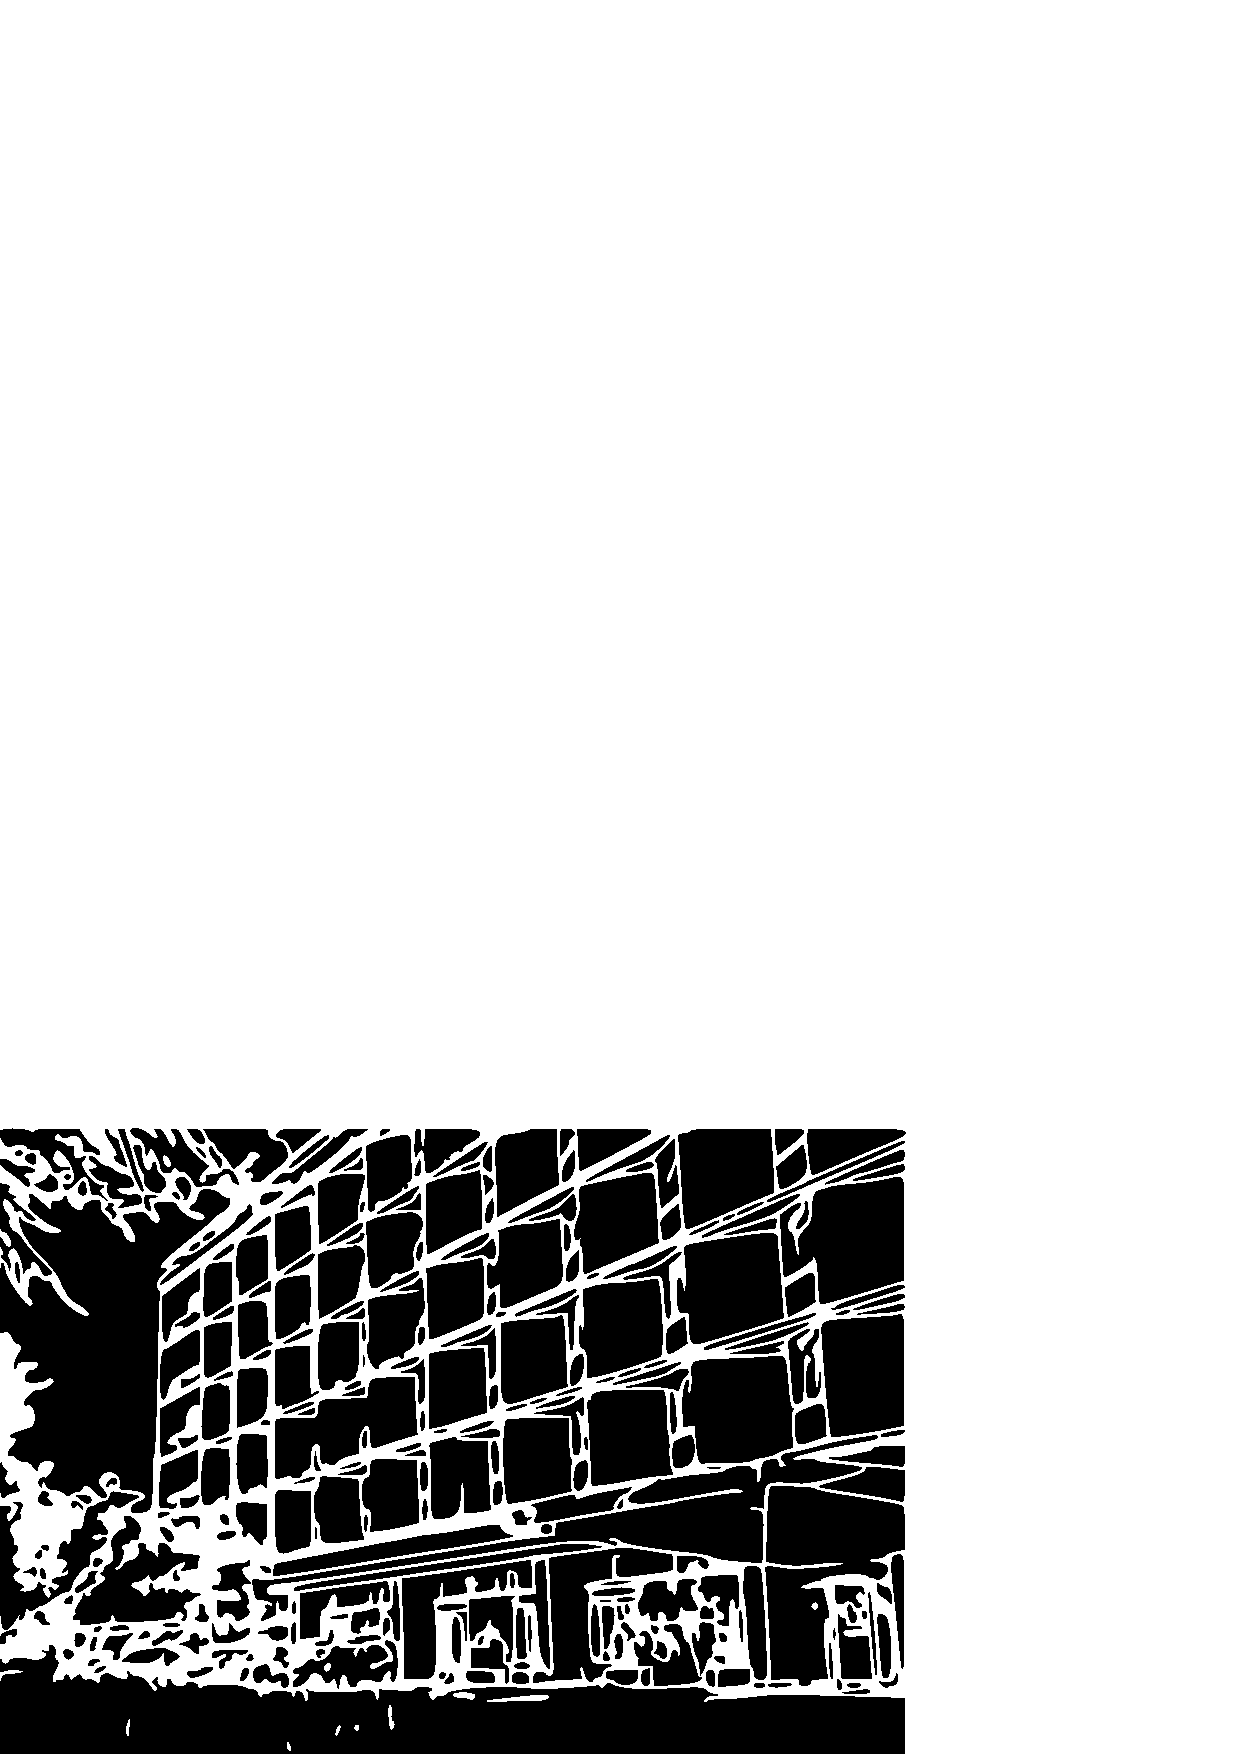
\includegraphics[width=0.45\textwidth]{Figures/building.jpg} &
        \includegraphics[width=0.45\textwidth]{Figures/Final.jpg} \\
    \end{tabular}
    \caption[Demonstration of full abstraction process]{Demonstration of full abstraction process. The final parameters and methods (of those under discussion) are a blur kernel of 5x5, a low threshold of 25 (for this example), Sobol seed point generation, and averaging via preliminary flood fill. It can be seen that most areas of the image are being effectively edge detected and flood filled with the correct colours; however, some areas are hard to interpret such as around the bushes in the bottom left, and some spaces have been left unfilled such as the panel below the top left corner of the building. These issues are minimal though, therefore leading me to conclude that the process is effective at producing recognisable abstractions of the input images.}
    \label{fig:Final}
    \end{center}
\end{figure}
        
\begin{figure}[ht]
    \begin{center}
    \begin{tabular}{ c c }
        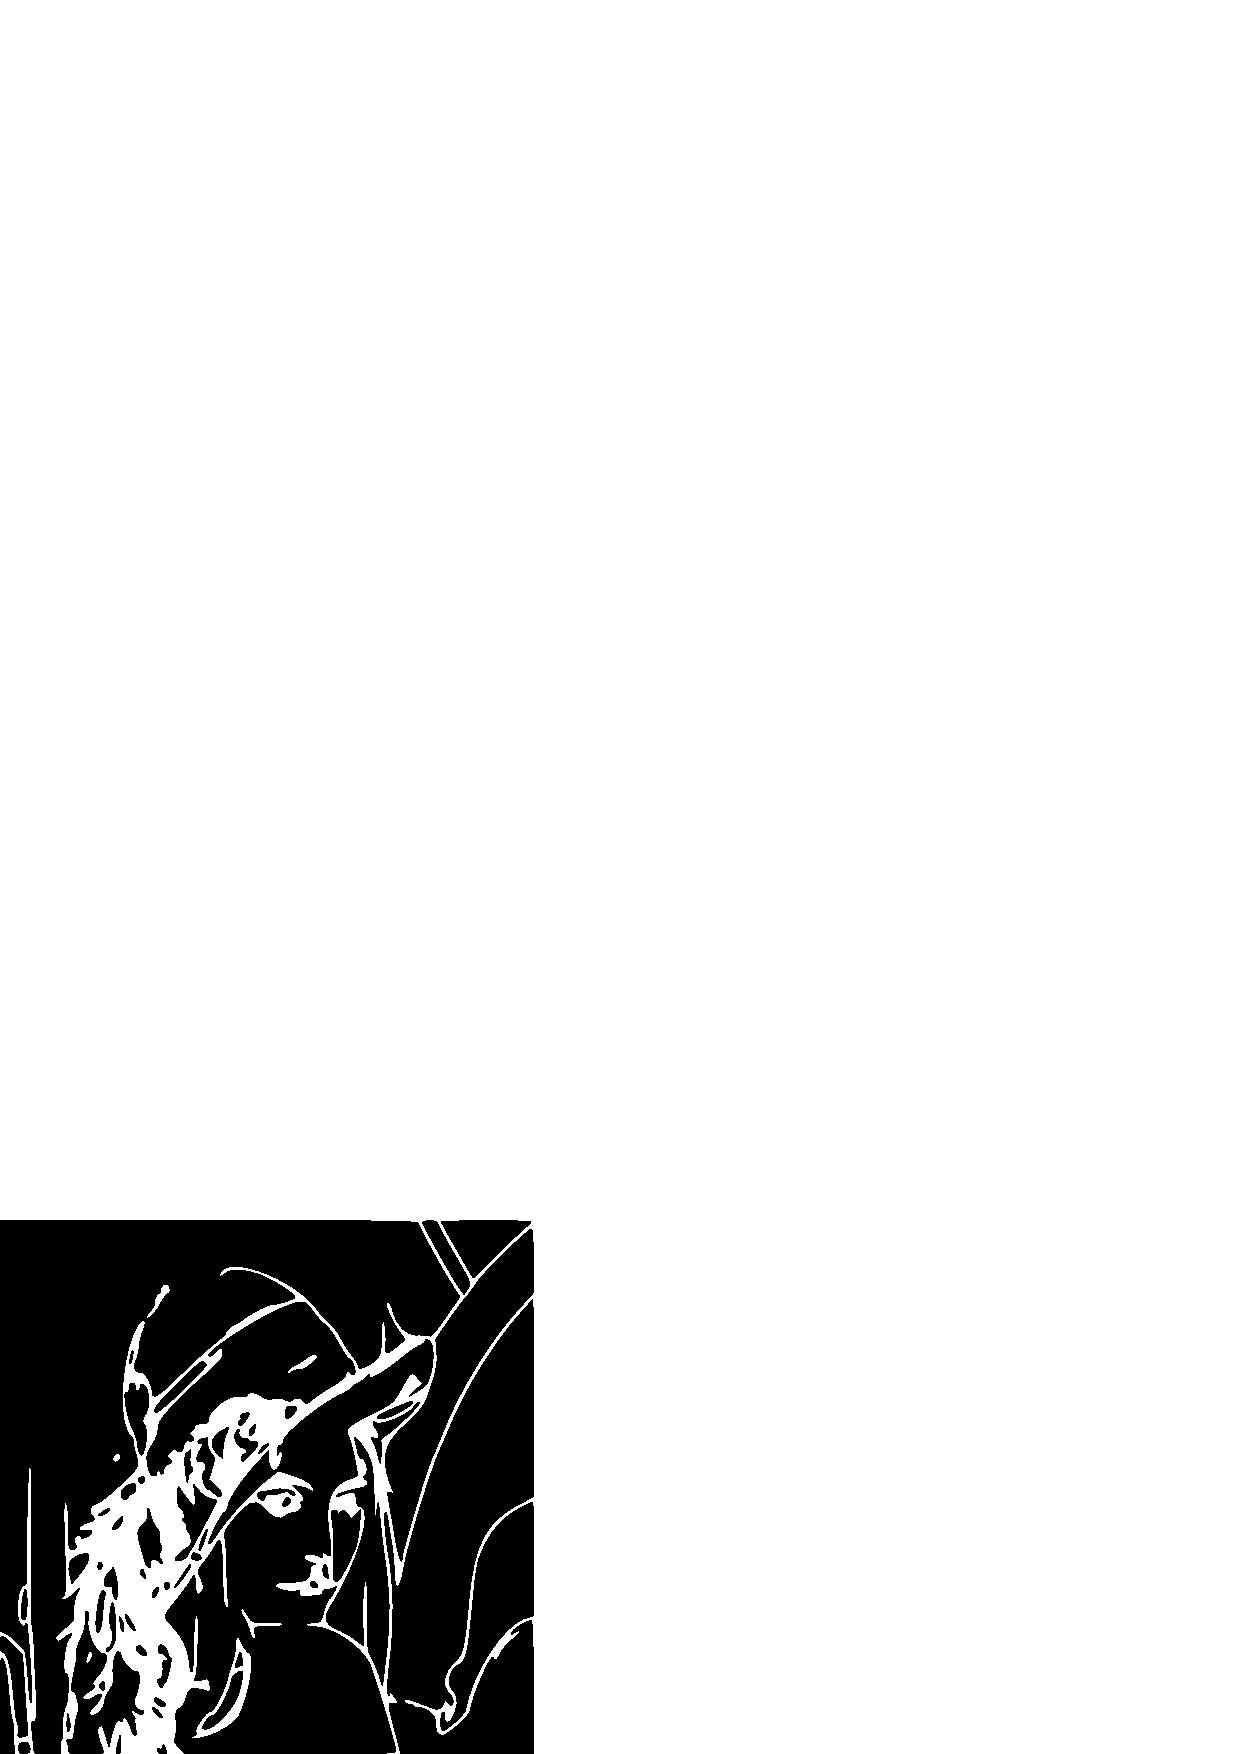
\includegraphics[width=0.43\textwidth]{Figures/lena.jpg} &
        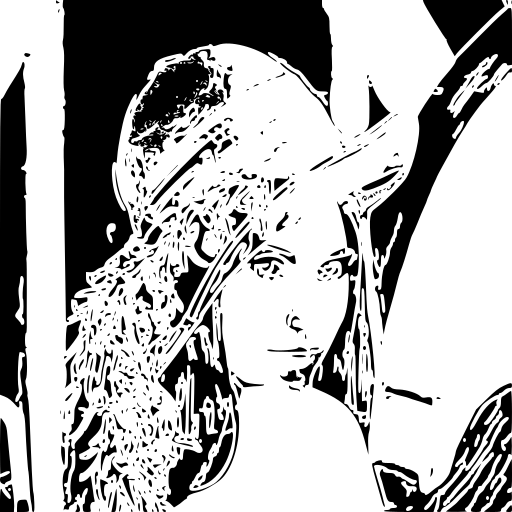
\includegraphics[width=0.43\textwidth]{Figures/lenaDA.jpg} \\
        \includegraphics[width=0.43\textwidth]{Figures/pufferfish6.jpg} &
        \includegraphics[width=0.43\textwidth]{Figures/pufferfishDA.jpg} \\
        \includegraphics[width=0.43\textwidth]{Figures/starry_night.jpg} &
        \includegraphics[width=0.43\textwidth]{Figures/starry_nightDA.jpg} 
    \end{tabular}
    \caption[Additional examples of the full abstraction process]{Additional examples of the full abstraction process. The top image (provided by OpenCV) is very simple, so the abstraction gives clean and easily recognisable results. The middle image (provided by fellow student Tom Darlison) was selected due to its limited colour palette and poor focus to test the limits of the process. While the image has mostly filled to a single colour, the pufferfish, rocks, coral, background fish, and open water are all identifiable. The bottom image (provided by OpenCV) was selected due to the extreme number of edges, due to the very clear brush strokes. Once the Canny threshold was turned down considerably, the result was recognisable as Starry Night, though much of the image has been overwhelmed by the edge detection lines. It can be concluded from these tests that the data abstraction process is effective at producing recognisable images, however the difficulty in interpreting the abstracted images is heavily dependant on the focus and complexity of the image.}
    \label{fig:FinalExtras}
    \end{center}
\end{figure} % Appendix Title
	
\chapter{Contour Based Seed Point Location}
\lhead{\emph{Contour Based Seed Point Location}}

The ideal place to aim to flood fill a space from would be the centre point of the space. OpenCV provides the functionality to take the Canny output image (a matrix of colour values) and convert it into a set of contours. Contours are line objects stored in a hierarchical structure and have functions that can provide the centre point of each contour. Although the centre points of the contours will not map exactly to the centre points of the space, they are close enough approximations to flood fill from (Figure \ref{fig:ContourCentres}).

Unfortunately, due to a combination of the processing time required to convert the lines into contours and the number of contours produced that have no impact on the spaces left to be flood filled, this method is too resource heavy to produce 10 fps on a laptop, therefore is also too resource heavy for use on the raspberry pi.

\begin{figure}[H]
    \begin{center}
    \begin{tabular}{ c c }
        
\includegraphics[width=0.31\textwidth]{Figures/blox.jpg} &
        \includegraphics[width=0.31\textwidth]{Figures/ContourCentres.jpg}
    \end{tabular}
    \caption[Demonstration of contour centre point location]{Demonstration of contour centre point location. The original image (provided by OpenCV) on the left has been Canny edge detected, these edges have converted into contours, and the centre points of these contours located. The results of this are displayed on the right, with each contour and its corresponding centre point in a different colour. It can be observed that the centre points provide adequate coverage of the black spaces in the image to be used as seed points for flood filling.}
    \label{fig:ContourCentres}
    \end{center}
\end{figure}
 % Appendix Title

\chapter{Images of Algorithm Performance Test Scenes}
\lhead{\emph{Images of Algorithm Performance Test Scenes}}
\label{Appendix:scenes}
        
\begin{figure}[ht]
    \begin{center}
    \begin{tabular}{ c }
        \includegraphics[width=0.6\textwidth]{Figures/simple.jpg} \\
        \includegraphics[width=0.6\textwidth]{Figures/medium.jpg} \\
        \includegraphics[width=0.6\textwidth]{Figures/complex.jpg} 
    \end{tabular}
    \caption[Images of Algorithm Performance Test Scenes]{Images of Algorithm Performance Test Scenes. From top to bottom, these are images of the simple scene, medium scene, and complex scene.}
    \label{fig:scenes}
    \end{center}
\end{figure} % Appendix Title

\chapter{Rover Hardware Breakdown}
\lhead{\emph{Rover Hardware Breakdown}}
\label{appendix:hardware}

\begin{table}[H]
\centering
\caption{List of all the components that make up the rover. Items listed as UoS were supplied by the University of Southampton.}
\label{table:hardware}
\resizebox{\textwidth}{!}{
\begin{tabular}{|l|l|l|l|}
\hline
Component              & Description                       & Quantity & Source           \\ \hline
Raspberry Pi 3         & Main computer                     & 1        & UoS              \\
ATmega644P             & Generates PWM for stepper drivers & 1        & UoS				 \\
Pololu DRV8825         & Stepper motor drivers             & 2        & HobbyTronics     \\
RS 535-0372            & Y-axis stepper motor              & 1        & Previous Project \cite{gimble} \\
SY35ST26-0284A         & X-axis stepper motor              & 1        & Previous Project \cite{gimble} \\
PlayStation 3 Eye      & Cameras                           & 2        & Amazon           \\
MAX14870               & DC motor drivers                  & 2        & HobbyTronics     \\
Lynxmotion GHM-04      & Drive motors                      & 4        & UoS				 \\
GEP-XT60-PDB           & Power distribution board          & 1        & Hobby King       \\
Turnigy 2650mAh 4S 20C & Lipo Batteries                    & 2        & Hobby King       \\
IC 108TTA050M 		   & Decoupling capacitors             & 2        & UoS				 \\ \hline
\end{tabular}}
\end{table}

\chapter{Vectorization}
\lhead{\emph{Vectorization}}
\label{appendix:vectorization}

As edge detected images consist of white lines on a black background, it would be logical to consider vector graphics as a storage method for wireless transmission. Vector graphics is the storage of images as line drawing and space filling instructions, allowing scaling to any size. When testing this, Potrace \cite{potrace} was used to convert the edge detected image bitmaps into encapsulated postscript documents (Figure \ref{fig:potrace}). 

\begin{figure}[H]
    \begin{center}
    \begin{tabular}{ c c }
        \multicolumn{2}{c}{\includegraphics[width=0.4\textwidth]{Figures/butterfly.jpg}} \\
        \includegraphics[width=0.4\textwidth]{Figures/butteredge.jpg} &
        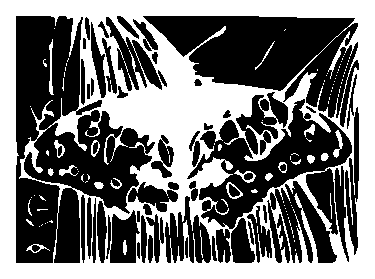
\includegraphics[width=0.4\textwidth]{Figures/butter.eps}
    \end{tabular}
    \caption[Conversion to Vector Graphics]{Conversion to Vector Graphics. While the vectorised image (bottom right) is clearly of the edge detection (bottom left), it utilises heavy approximation.}
    \label{fig:potrace}
    \end{center}
\end{figure}

When the documents were received by the server, they were converted back to OpenCV bitmaps using a custom interpreter built for the project. Both due to the approximation applied by Potrace and the custom interpreter not including all the necessary functions to accurately convert the vector files back to bitmaps, the final result loses much of its accuracy to the original image (Figure \ref{fig:potracecomp}). Due to the high edge accuracy requirements of producing a depth map from edge detected images, this method was discarded in favour of standard image compression. 

\begin{figure}[H]
    \begin{center}
    \begin{tabular}{ c c }
        \includegraphics[width=0.4\textwidth]{Figures/buttercan.jpg} &
        \includegraphics[width=0.4\textwidth]{Figures/butterred.jpg}
    \end{tabular}
    \caption[Comparison of Vector and Bitmap Accuracy]{Comparison of Vector and Bitmap Accuracy. Once the vector image has been converted back into a bitmap (right), it has lost much of its resemblance to the original image. A comparison to the image that results from transmitting compressed bitmaps (left) shows the sheer number of edges that have been either lost or combined together.}
    \label{fig:potracecomp}
    \end{center}
\end{figure}

\chapter{Project Brief}
\lhead{\emph{Project Brief}}
\label{appendix:brief}

\begin{center}
\textbf{Using Data Abstraction and Inter-Frame Interpolation for Low Data Rate Communication Between a 3D Camera and VR Headset} \\
Adam Melvin am20g15@soton.ac.uk \\
Klaus-Peter Zauner kpz@soton.ac.uk
\end{center}

There are many challenges, such as monitoring hostile environments, that call for the use of remotely controlled robots. Often in these scenarios, it would be useful to be able to view the environment with a sense of depth to better understand the scale, and dangers, of the robot’s surroundings. This can be provided through the use of a 3D camera on the robot and Virtual Reality (VR) goggles, however due to the minimum frame rate that can be displayed in a VR headset without causing motion sickness in the user being 60fps (optimally 90fps is preferable), a comfortable and useful experience would often require an unfeasibly high wireless data rate.

The aim of this project is to significantly reduce the data rate required to be transmitted between a robot and teleoperator through the use of data abstraction and inter-frame interpolation. A 3D camera rig mounted on a remotely controlled rover is to take around 10 pictures per second, then they are reduced down to the minimum amount of data required to identify the objects in the environment. These much smaller images are sent wirelessly to a server, where they are used to create a 3D map of the environment. These 3D maps are analysed and intermediate frames are estimated to increase the frame rate from 10fps to 60-90fps. This much higher frame rate estimated map of the environment can then be displayed in the VR headset through the use of a video game engine. Although the estimated frames will not accurately represent the real world, the comfort they provide the user will allow them to focus on the transmitted information without feeling ill.

A simple rover and off-the-shelf VR equipment will be used as a foundation for the system. Different camera systems and interpolation algorithms will be tested on this foundation to discern the setup that produces the best ratio between data rate and usability.


\chapter{Gantt Charts}
\lhead{\emph{Gantt Charts}}
\begin{landscape}
\begin{figure}[ht]
    \begin{center}
    \includegraphics[width=1.5\textwidth]{Figures/ganttfinal.png}
    \label{fig:GanttChart}
    \end{center}
\end{figure}
\end{landscape} % Appendix Title

\chapter{Risk Assessment}
\lhead{\emph{Risk Assessment}}

\begin{figure}[H]
    \begin{center}
      \includegraphics[width=\textwidth]{Figures/RiskAssessment.png}
      \caption[Risk Assessment]{Risk Assessment for the project going forward.}
      \label{fig:Risk}
    \end{center}
\end{figure} % Appendix Title

\chapter{Design Archive Contents}
\lhead{\emph{Design Archive Contents}}
\label{appendix:archive}

\begin{forest}
  for tree={
    font=\ttfamily,
    grow'=0,
    child anchor=west,
    parent anchor=south,
    anchor=west,
    calign=first,
    inner xsep=7pt,
    edge path={
      \noexpand\path [draw, \forestoption{edge}]
      (!u.south west) +(7.5pt,0) |- (.child anchor) pic {} \forestoption{edge label};
    },
    before typesetting nodes={
      if n=1
        {insert before={[,phantom]}}
        {}
    },
    fit=band,
    before computing xy={l=15pt},
  }  
[DesignArchive
  [CompressionTests
  	[imagequant
  	]
  	[PotraceImage
  	]
  ]
  [CVTests
    [AbstractWCamNCircleAverage
    ]
    [AbstractWCircleAverage
    ]
    [AverageColour
    	[1Point
    	]
    	[2Circle
    	]
    	[3Flood
    	]
    ]
    [Contours
    ]
    [DepthMap
    ]
    [FrameRate
    ]
    [LibelasTest
    ]
  ]
  [Hardware
  ]
  [Images
  ]
]
\end{forest}
\begin{forest}
  for tree={
    font=\ttfamily,
    grow'=0,
    child anchor=west,
    parent anchor=south,
    anchor=west,
    calign=first,
    inner xsep=7pt,
    edge path={
      \noexpand\path [draw, \forestoption{edge}]
      (!u.south west) +(7.5pt,0) |- (.child anchor) pic {} \forestoption{edge label};
    },
    before typesetting nodes={
      if n=1
        {insert before={[,phantom]}}
        {}
    },
    fit=band,
    before computing xy={l=15pt},
  }  
[
  [FinalBuilds
  	[Abstraction
  		[Camera
  		]
  		[Image
  		]
  	]
  	[RoverToUbuntu
  		[Rover
  		]
  		[UbuntuServer
  		]
  	]
  	[RoverToUnreal
  		[Rover
  		]
  		[UnrealComponents
  		]
  	]
  ]
  [UDPTests
  	[CamReceive
  	]
  	[CamSend
  	]
  	[CamSendThreaded
  	]
  	[ImageReceive
  	]
  	[ImageSend
  	]
  ]
]
\end{forest}
\clearpage
\begin{forest}
  for tree={
    font=\ttfamily,
    grow'=0,
    child anchor=west,
    parent anchor=south,
    anchor=west,
    calign=first,
    inner xsep=7pt,
    edge path={
      \noexpand\path [draw, \forestoption{edge}]
      (!u.south west) +(7.5pt,0) |- (.child anchor) pic {} \forestoption{edge label};
    },
    before typesetting nodes={
      if n=1
        {insert before={[,phantom]}}
        {}
    },
    fit=band,
    before computing xy={l=15pt},
  }  
[
  [SystemTests
  	[FPSTest
  	]
  	[JPGSystem
  		[rover
  		]
  		[server
  		]
  	]
  ]
]
\end{forest} % Appendix Title


\end{document}  % The End
%% ----------------------------------------------------------------